\documentclass[a4paper, 12pt]{article}
\usepackage[a4paper,top=1.5cm, bottom=1.5cm, left=1cm, right=1cm]{geometry}
\usepackage{cmap}					
\usepackage{mathtext} 				
\usepackage[T2A]{fontenc}			
\usepackage[utf8]{inputenc}			
\usepackage[english,russian]{babel}
\usepackage{multirow}
\usepackage{graphicx}
\documentclass{article}
\usepackage{listings}
\usepackage{xcolor}
\graphicspath{ {./images/} }
\usepackage{wrapfig}
\usepackage{tabularx}
\usepackage{float}
\usepackage{longtable}
\usepackage{hyperref}
\hypersetup{colorlinks=true,urlcolor=blue}
\usepackage[rgb]{xcolor}
\usepackage{amsmath,amsfonts,amssymb,amsthm,mathtools} 
\usepackage{icomma} 
\usepackage{euscript}
\usepackage{mathrsfs}
\usepackage{enumerate}
\usepackage{caption}
\usepackage{enumerate}
\usepackage{graphicx}
\usepackage{caption}
\usepackage{subcaption}
\usepackage[europeanresistors, americaninductors]{circuitikz}
\DeclareMathOperator{\sgn}{\mathop{sgn}}
\newcommand*{\hm}[1]{#1\nobreak\discretionary{}
	{\hbox{$\mathsurround=0pt #1$}}{}}
\title{\textbf{Лабораторная работа по float}}
\author{Моргулёв Илья}
\date{Октябрь 10, 2023}
\begin{document}
    \maketitle

    \section{Введение.}

    \textbf{Цель работы:} ознакомление с хранением чисел типа float в памяти компьютера и изучение закономерностей с этим связанных.
    \bigskip\\
    \textbf{Оборудование:} Ноутбук, программы для воспроизведения, компиляции и дебаггинга кода, онлайн компиляторы и строители графиков.

    \section{Теоретические сведения.}
        Float - формат чисел с плавающей точкой. В связи с чем возникают особенности: хранение с помощью мантисы позволяет с высокой степнью точности считать многие вещественные числа, вместе с чем возникают некоторые трудности: переполнение мантисы, приближённое число и прочее.
        \[\]
        Union - это оператор в языке SQL, применяется для объединения двух наборов строк, возвращаемых SQL-запросами. Оба запроса должны возвращать одинаковое число столбцов, и столбцы с одинаковым порядковым номером должны иметь совместимые типы данных. (пример: см. Задание 1)
        \[\]
        IEEE 754-2008 - это правило, по которому компьютер высчитывает число и хранит его. 
        \[
        Number_{10} = (-1)^s \cdot 2^{E-127} \cdot (1+\frac{m}{2^n})
        \] Где $S$ - бит знака (0 - положительное; 1 - отрицательное), $E$ - смещённая экспонента двоичного числа, $m$ - остаток мантисы двоичного двоичного нормализованного числа.

    \section{Ход работы}
    \begin{enumerate}
        \item \textbf{Задание 0:} Вывести на экран unsigned int в двоичной системе счисления (то есть так, как этот unsigned int хранится в памяти компьютера), используя побитовые операции.

        \lstset { %
        language=C++,
        backgroundcolor=\color{black!5}, % set backgroundcolor
        basicstyle=\footnotesize,% basic font setting
        }
        Используемый код:
        \begin{lstlisting}
        #include <iostream>
        using namespace std;

        int main(){
            unsigned int n,k,b;
            int a =0;
            cin >> n;
            k=1;
            k<<=31;
            for (int i=0;i<32;i++){
                b=n&k;
                if (b == 0) cout << 0;
                else cout << 1;
                k>>=1;
                if (a==3) {cout << " "; a=0;}
                else a++;
            }
        }
        \end{lstlisting}

        Программа роботает, выводит число в том виде, как оно хранится в компьютере, перепишем функцию $main$ в вызываемую функцию $binary$.

        \item \textbf{Задание 1:} С помощью union и функции из предыдущего пункта вывести на экран представление float в памяти компьютера. Проверьте, что $IEEE 754-2008$ (стандарт) действительно работает.

        \lstset { %
            language=C++,
            backgroundcolor=\color{black!5}, % set backgroundcolor
            basicstyle=\footnotesize,% basic font setting
        }
        Используемый код:
        \begin{lstlisting}
        #include <iostream>
        union flo_int{
            unsigned int u;
            float f;
        };
        void binary(unsigned int n){
            unsigned int k,b;
            int a =0;
            k=1;
            k<<=31;
            for (int i=0;i<32;i++){
                b=n&k;
                if (b == 0) std::cout << 0;
                else std::cout << 1;
                k>>=1;
                if (a==3) {std::cout << " "; a=0;}
                else a++;
            }
        }
        int main(){
            flo_int n_lab_rat;
            std::cin >> n_lab_rat.f;
            binary(n_lab_rat.u);
        }
        \end{lstlisting}
        

        Убедимся в соответствии (или несоответсвии):
        
        \begin{tabular}{|c|c|c|}
            \hline
            ввод & вывод & $IEEE 754-2008$ \\\hline
            5 & 0100 0000 1010 0000 0000 0000 0000 0000 & Соответствует\\\hline
            12.5 & 0100 0001 0100 1000 0000 0000 0000 0000 & Соответствует\\\hline
            37.5 & 0100 0010 0001 0110 0000 0000 0000 0000 & Соответствует\\\hline
            101.567 & 0100 0010 1100 1011 0010 0010 0100 1110 & Соответствует\\\hline
            123.5 & 0100 0010 1111 0111 0000 0000 0000 0000 & Соответствует\\\hline
            12345.23456 & 0100 0110 0100 0000 1110 0100 1111 0000 & Сооветствует\\\hline
            -123.456 & 0100 0110 0100 0000 1110 0100 1111 0000 & Соответствует\\\hline
        \end{tabular}
        \newpage
        \item \textbf{Задание 2:} Воспроизвести переполнение мантиссы. Проще и нагляднее всего – в цикле выводить десятичное и двоичное представление степеней десятки.

        \lstset { %
            language=C++,
            backgroundcolor=\color{black!5}, % set backgroundcolor
            basicstyle=\footnotesize,% basic font setting
        }
        Используемый код:
        \begin{lstlisting}
        #include <iostream>
        union flo_int{
            unsigned int u;
            float f;
        };
        void binary(unsigned int n){
            unsigned int k,b;
            int a =0;
            k=1;
            k<<=31;
            for (int i=0;i<32;i++){
                b=n&k;
                if (b == 0) std::cout << 0;
                else std::cout << 1;
                k>>=1;
                if (a==3) {std::cout << " "; a=0;}
                else a++;
            }
        }
        int main(){
            std::cout << std::fixed;
            std::cout.precision(2);
            flo_int n_lab_rat;
            float k =1.0;
            for (int i=0;i<39;i++){
                n_lab_rat.f=k*10;
                k*=10;
                std::cout << k/10 << " // ";
                binary(n_lab_rat.u);
                std::cout << std::endl;
            }
        }
        \end{lstlisting}
        Проанализируем выходные данные, занесённые в таблицу:
        
        \begin{tabular}{|l|l|}
        \hline
        1.00                          & 0100 0001 0010 0000 0000 0000 0000 0000 \\
        10.00                         & 0100 0010 1100 1000 0000 0000 0000 0000 \\
        100.00                        & 0100 0100 0111 1010 0000 0000 0000 0000 \\ \cline{1-1}
        \multicolumn{1}{|l|}{1000.00} & 0100 0110 0001 1100 0100 0000 0000 0000 \\ \cline{1-1}
        10000.00                      & 0100 0111 1100 0011 0101 0000 0000 0000 \\
        100000.00                     & 0100 1001 0111 0100 0010 0100 0000 0000 \\
        1000000.00                    & 0100 1011 0001 1000 1001 0110 1000 0000 \\
        10000000.00                   & 0100 1100 1011 1110 1011 1100 0010 0000 \\
        100000000.00                  & 0100 1110 0110 1110 0110 1011 0010 1000 \\
        1000000000.00                 & 0101 0000 0001 0101 0000 0010 1111 1001 \\
        10000000000.00                & 0101 0001 1011 1010 0100 0011 1011 0111 \\
        99999997952.00                & 0101 0011 0110 1000 1101 0100 1010 0101 \\
        999999995904.00               & 0101 0101 0001 0001 1000 0100 1110 0111 \\
        9999999827968.00              & 0101 0110 1011 0101 1110 0110 0010 0001 \\
        100000000376832.00            & 0101 1000 0110 0011 0101 1111 1010 1001 \\
        1000000054099968.00           & 0101 1010 0000 1110 0001 1011 1100 1010 \\
        10000000272564224.00          & 0101 1011 1011 0001 1010 0010 1011 1100 \\
        99999998430674944.00          & 0101 1101 0101 1110 0000 1011 0110 1011 \\
        999999984306749440.00         & 0101 1111 0000 1010 1100 0111 0010 0011 \\
        9999999980506447872.00        & 0110 0000 1010 1101 0111 1000 1110 1100 \\\hline
        \end{tabular}
        
        Как мы видим, из-за особенностей записи числа типа $float$ в памяти компьютера возникает ситуация, что в мантиссе возникают значащие единицы, которые привлдят в последствии умножения на 10 к тому, что число не совсем уж и умножается на 10. Пример - $10000000000.00 -> 99999997952.00$ - умножение на 10 выглядит немного странно, согласитесь. В следствие того, что единица в бинарном разлодении будто "вылазиет" из мантиссы это и названно переполнением мантисы.  
        \[\]
        \item \textbf{Задание 3:} Создать бесконнечный цикл.
        \[\]
        \lstset { %
            language=C++,
            backgroundcolor=\color{black!5}, % set backgroundcolor
            basicstyle=\footnotesize,% basic font setting
        }
        Используемый код:
        \begin{lstlisting}
        #include <iostream>
        
        int main(){
            std::cout << std::fixed;
            std::cout.precision(2);
            float f;
            int k=0;
            system("color 02");
            std::cin >> f;
            for (f;f<10000000000;f++){
                std::cout << f << " -_//_- ";
                k++;
                if (k==5) {k=0; std::cout << std::endl;}
        
            }
        }
        \end{lstlisting}
        \bigskip
        На значении f, равном $16777216.00$ , расстояние между соседними $float f$ будет больше единицы, отчего после цикл не сможет "перепрыгнуть" с одной иттерации цикла на другую. Это происходит из-за того, что не все числа могут быть закодированны в мантисе. Простой пример - число $0.2$ , переводя его в $float$ получим следующую последовательность шагов:
        \[\]
        \begin{tabular}{|c|c|c|}
        \hline
        номер шага & текущее число & пояснение \\\hline
        \hline
        0 & 0.2 & non\\\hline
        1 & 0.4 & non\\\hline
        2 & 0.8 & non \\\hline
        3 & 1.6 & ->выделяем целую часть\\\hline
        3 & 0.6 & non\\\hline
        4 & 1.2 & ->выделяем целую часть\\\hline
        4 & 0.2 & non\\\hline
        \end{tabular}
        \[\]
        Как мы видим цикл записи числа $0.2$ перешёл в бесконечный цикл в связи с особенностями типа $float$. Что же тогда запишется в память компьютера? Число, приблизительно равное $0.2$ . В связи с этим, в довесок, появляются проблемы с сравнением чисел, но нас волнует число  $16777216.00$ . Так это число выглядит в памяти компьютера:
        \textbf{0100 1011 1000 0000 0000 0000 0000 0000} . 
        Однако следующее за ним число - $16777217.00$ имеет такой же двоичный код в памяти компьютера, следовательно прибавляя единицу к $16777216.00$ двоичный код не меняется и компьютер не видит разницы оставаясь на той же иттерации. Выражаясь неформально: компилятор не смог "перепрыгнуть" с одной иттерации на другую, так как с увличением числа типа $float$ между числами появлюятся некоторые зазоры, которые как раз и могут привести к подобному результату.
        \newpage
        \item \textbf{Задание 4:} График $\pi$.
        Найдём 4-5 иттерационных формул для числа $\pi$, посчитаем, построим график зависимости точности от количества иттераций. Найдём ошибку подсчёта.
                \bigskip
                \begin{enumerate}
                    \item[\textbf{1.1: }]  \textbf{Формула Лейбница.}
                        \begin{equation}
                            \pi = 4\sum \limits_{i=0}^{\infty} \frac{(-1)^i}{2i+1}
                        \end{equation}
                        
                        \lstset { %
                            language=C++,
                            backgroundcolor=\color{black!5}, % set backgroundcolor
                            basicstyle=\footnotesize,% basic font setting
                        }
                        Используемый код:
                        \begin{lstlisting}
                #include <iostream>
                #include <math.h>
                #include <fstream>
                using namespace std;                
                int main() {
                    float n;
                    float pi;
                    ofstream pi_res("1.csv", ios::out);
                    pi=0;    
                    std::cout << "Approx Leibnica's series\n";
                    std::cout << "\nEnter the number of iterations: ";
                    std::cin >> n;
                    std::cout << "Please wait. Running..." << "\n";            
                        for(long long int i = 0; i < n; i++){
                            if (i%2 == 0) pi+=4.0/((2.0*i) + 1.0);
                            else pi+=-4.0/((2.0*i) + 1.0);
                        pi_res << "[" << i << ", " << pi << "], ";
                       }
                   return 0;
                }
                        \end{lstlisting}
    
                        \begin{figure}[h!]
    			        \centering
    			            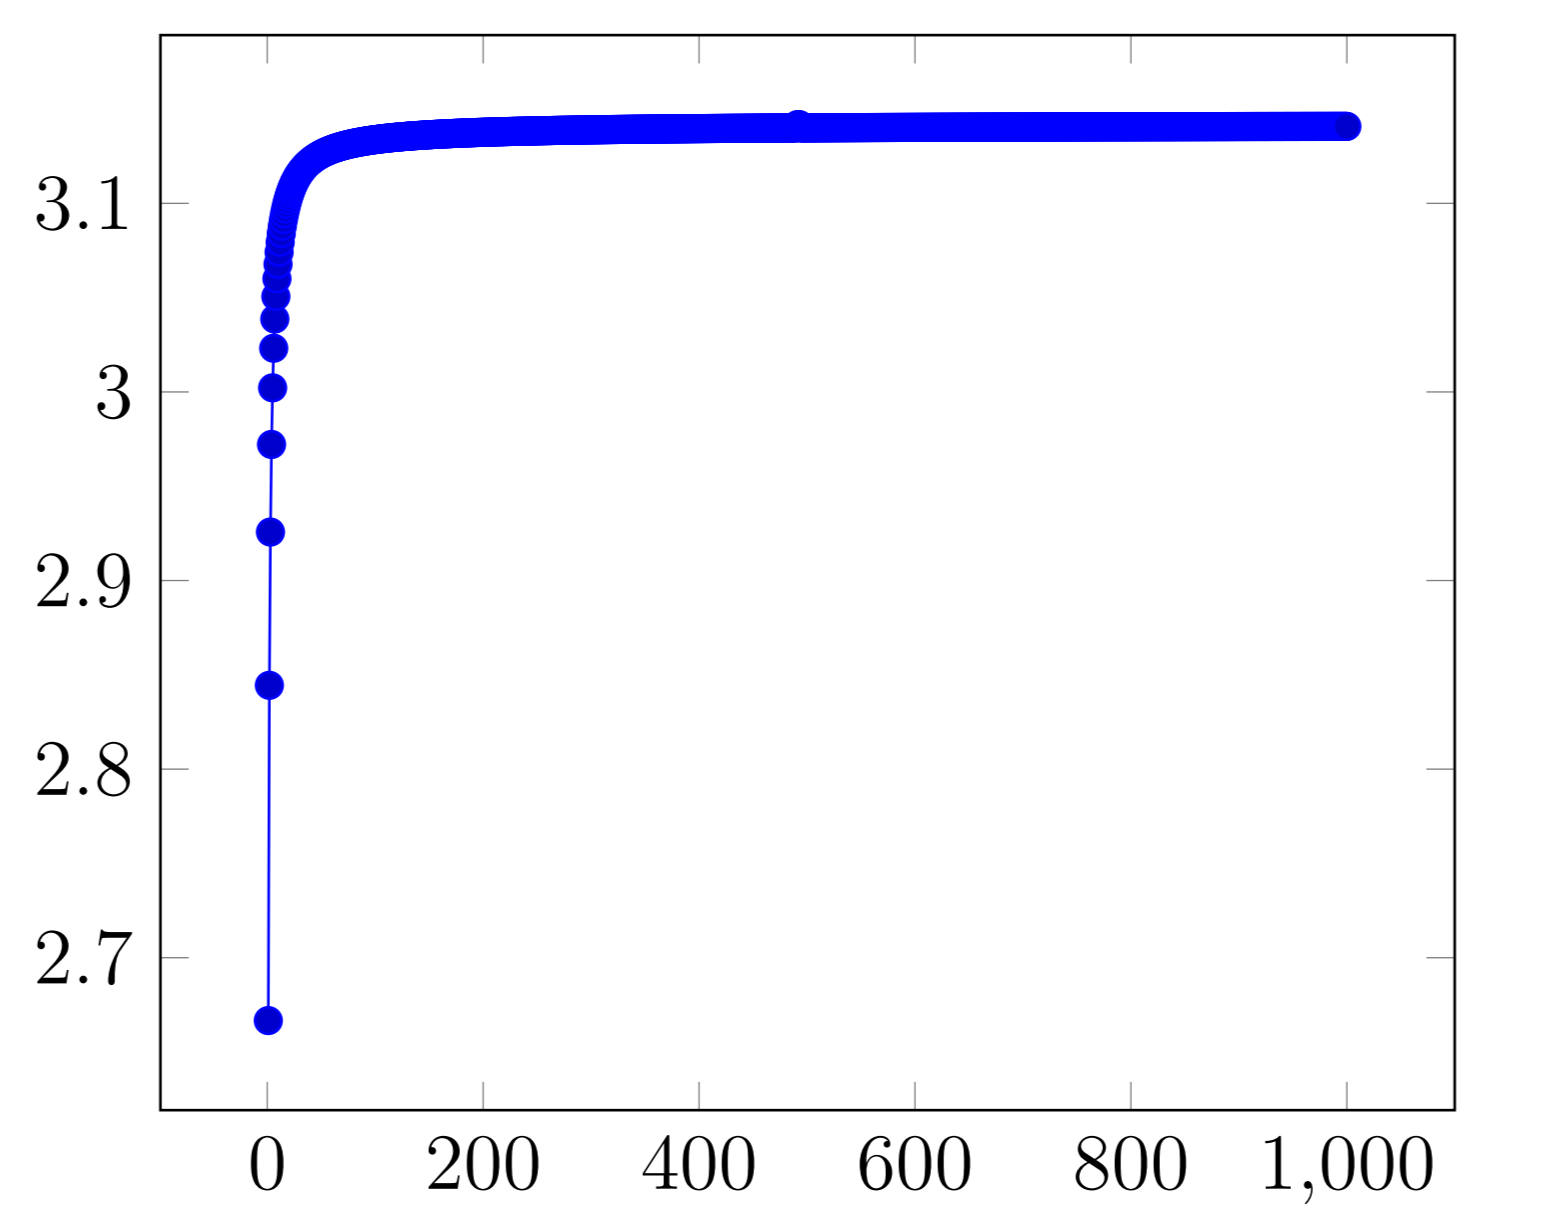
\includegraphics[scale = 0.25]{1-1.png}
    			            \caption{График зависимости числа $\pi$ от числа итераций ($n$)}
    			            \label{fig:my_label}
    		          \end{figure}
                        \bigskip
                        \begin{figure}[h!]
    			        \centering
    			            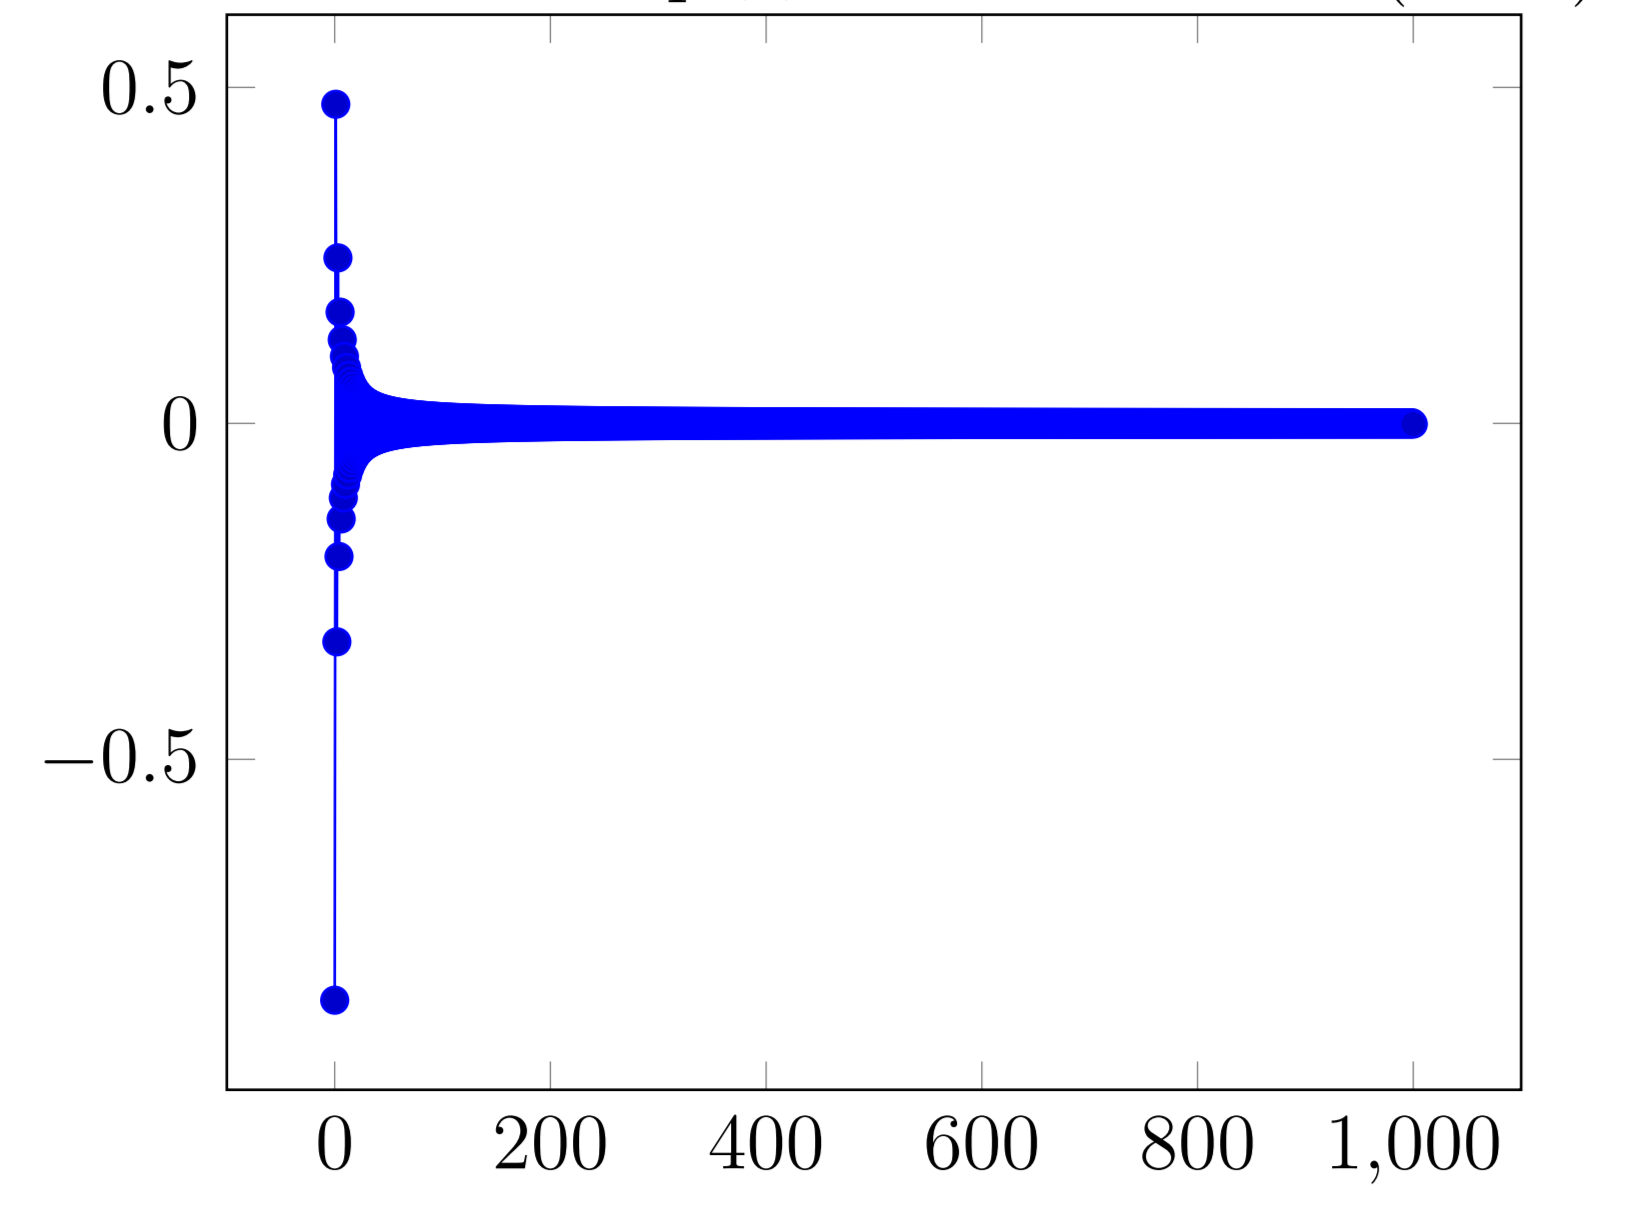
\includegraphics[scale = 0.3]{1-2.png}
    			            \caption{Разности истинного значения числа $\pi$ и полученного нами значения в формуле в зависимости от номера итерации}
    			            \label{fig:my_label}
    		          \end{figure}
                
                        \newpage
                        Рассмотрим участок времени от 0 до 60 итераций, рассмотрим, как ведёт себя разница между полученным нами значением и истинным значением:
                        \begin{figure}[h!]
    			        \centering
    			            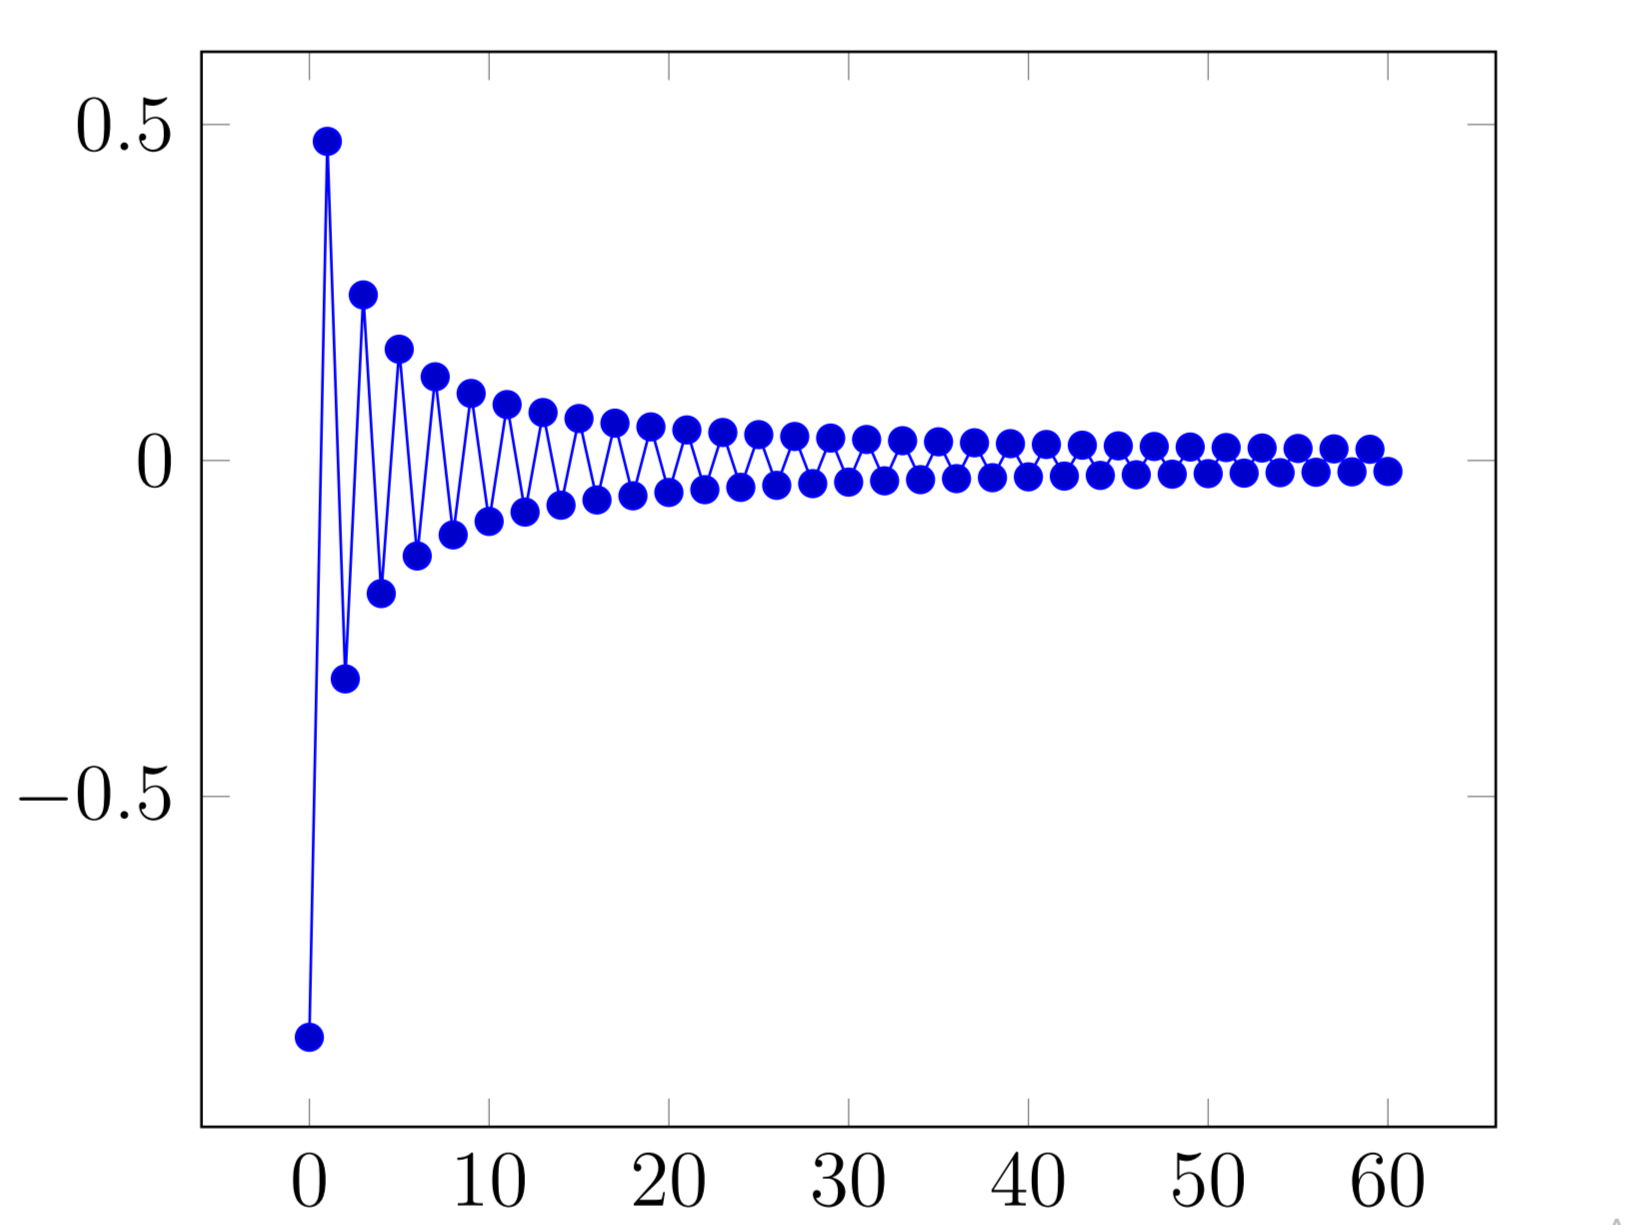
\includegraphics[scale = 0.18]{1-3.png}
    			            \caption{разница между полученным нами значением и истинным значением в зависимости от номера итерации}
    			            \label{fig:my_label}
    		          \end{figure}
                        \newpage
                        Как мы видим, последовательность полученных нами значений, сходится к истинному значению с двух сторон.
                        Рассмотрим участок от 500 до 1000:
                        \begin{figure}[h!]
    			        \centering
    			            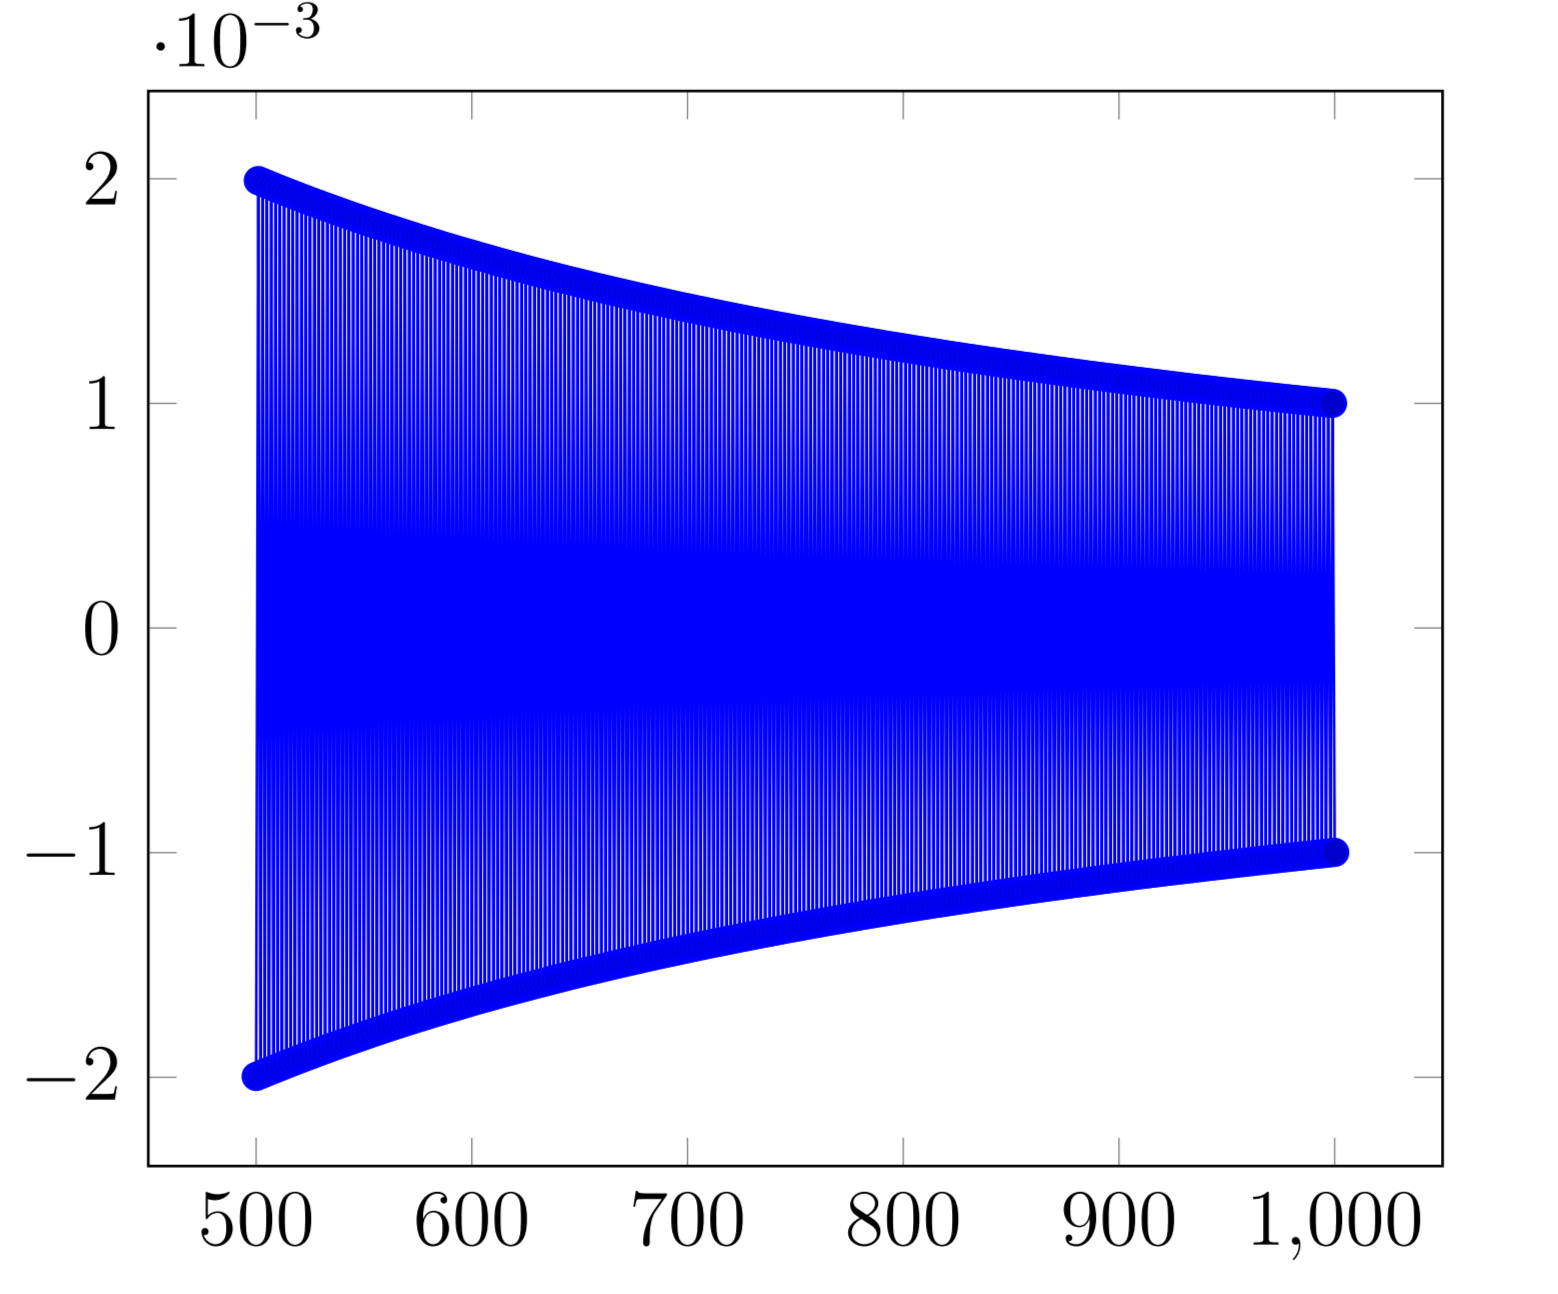
\includegraphics[scale = 0.3]{1-4.png}
    			            \caption{разница между полученным нами значением и истинным значением в зависимости от номера итерации}
    			            \label{fig:my_label}
    		          \end{figure}
                        \bigskip 
                        Как мы видим по графику (и что было вполне очевидно) - разность между истинным значением и полученным нами отличается на тысячные доли и колеблется вокруг истинного значения.
                        \[\]
                        \textbf{Следствие:} при измерении числа $\pi$ с помощью формулы (1) точность составляет ~0.0001.
                        \bigskip
                        
                    \newpage
                    \item[\textbf{1.2: }]  \textbf{Формула Валлиса.}
                            \begin{equation}
                                \pi = 2 \cdot \prod\limits_{i=0}^{\infty} \frac{4i^2}{4i^2-1}
                            \end{equation}
                            \lstset { %
                                language=C++,
                                backgroundcolor=\color{black!5}, % set backgroundcolor
                                basicstyle=\footnotesize,% basic font setting
                            }
                            Используемый код:
                            \begin{lstlisting}
                #include <iostream>
                #include <math.h>
                #include <fstream>
                using namespace std;            
                int main() {
                    float n, i, j;
                    float pi;
                    ofstream pi_res("1.csv", ios::out);
                    while (1){
                        pi=1.0;                            
                        std::cout << "PI through the Vallie's series\n";
                        std::cout << "\nEnter the number of iterations: ";
                        std::cin >> n;
                        std::cout << "Please wait. Running..." << "\n";
                        for (i=0;i<n;i++){
                            j=4.0*pow(i,2);
                            pi *= j/(j-1.0);
                            pi_res << "[" << i << ", " << pi << "], ";
                        }
                    }
                   return 0;
                }
                                                        
                            \end{lstlisting}
        
                            \begin{figure}[h!]
        			        \centering
        			            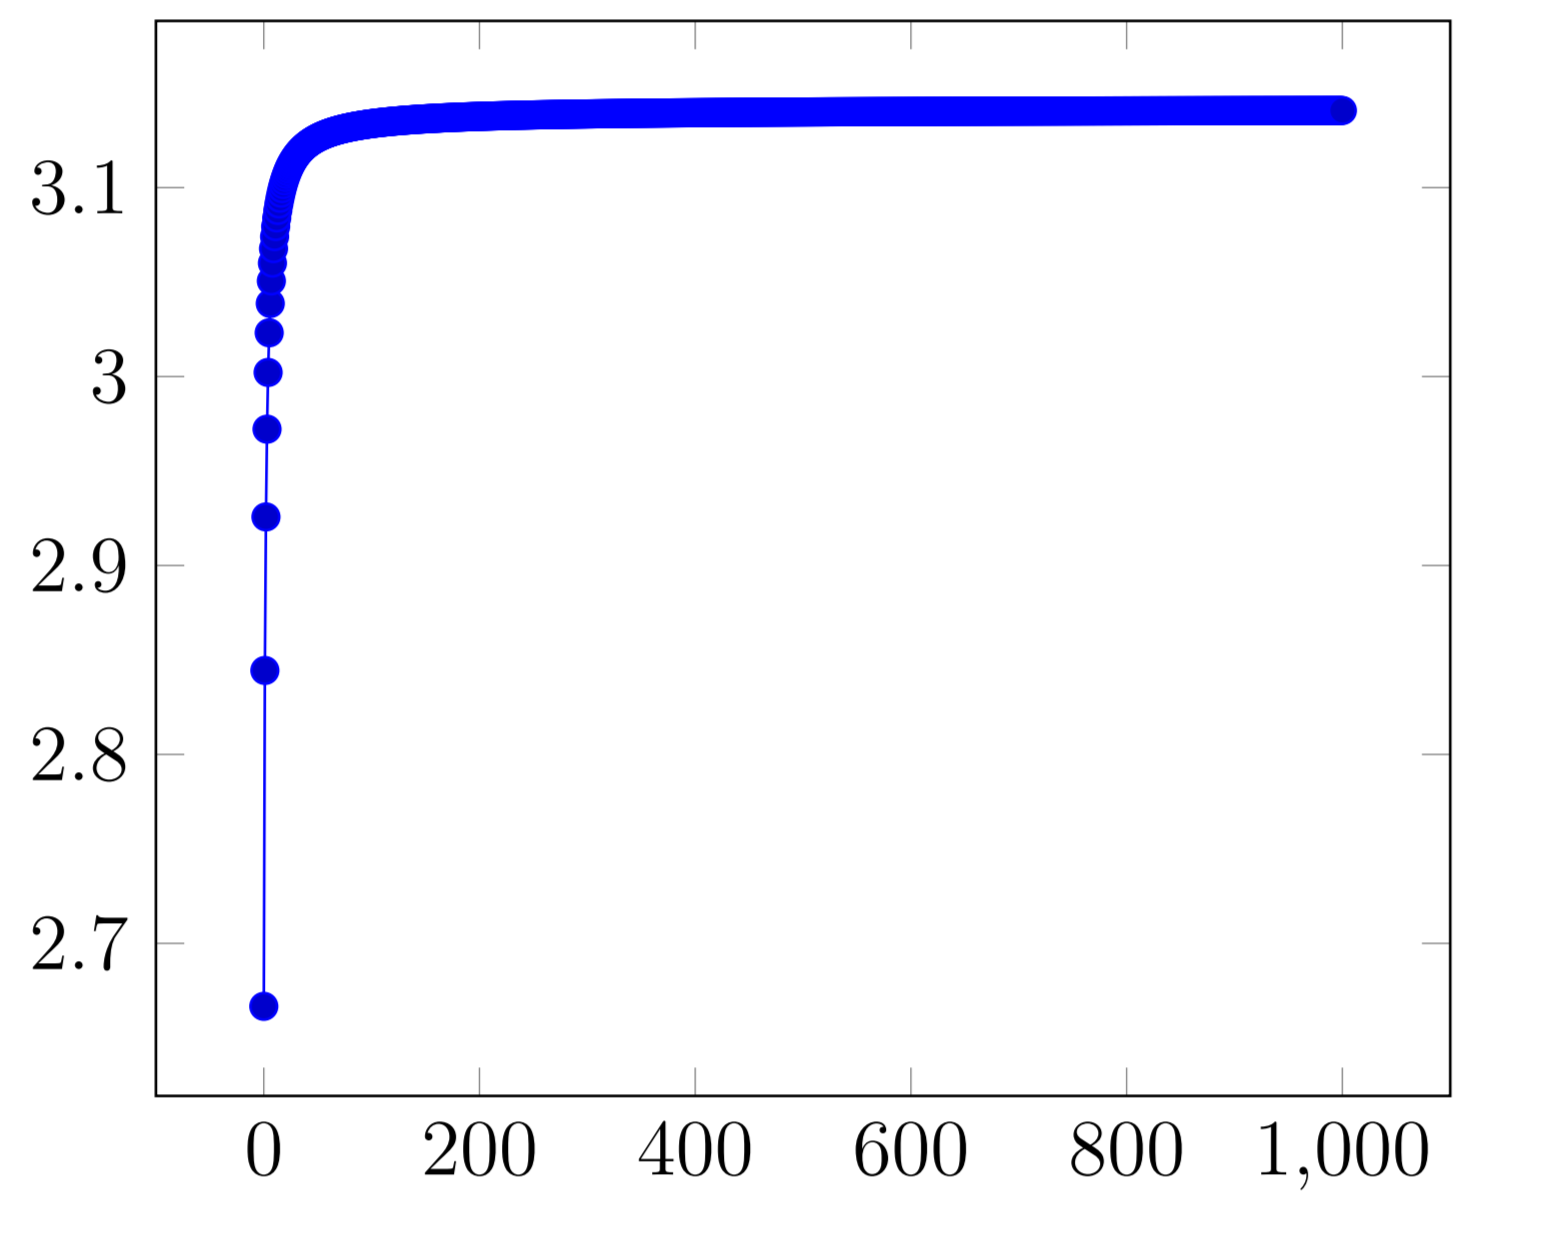
\includegraphics[scale = 0.25]{2-1.png}
        			            \caption{График зависимости числа $\pi$ от числа итераций ($n$)}
        			            \label{fig:my_label}
        		          \end{figure}
                            \newpage
                            Рассмотрим разность между истинным значением числа $\pi$ и полученным нами с помощью формулы (2):
                            \begin{figure}[h!]
        			        \centering
        			            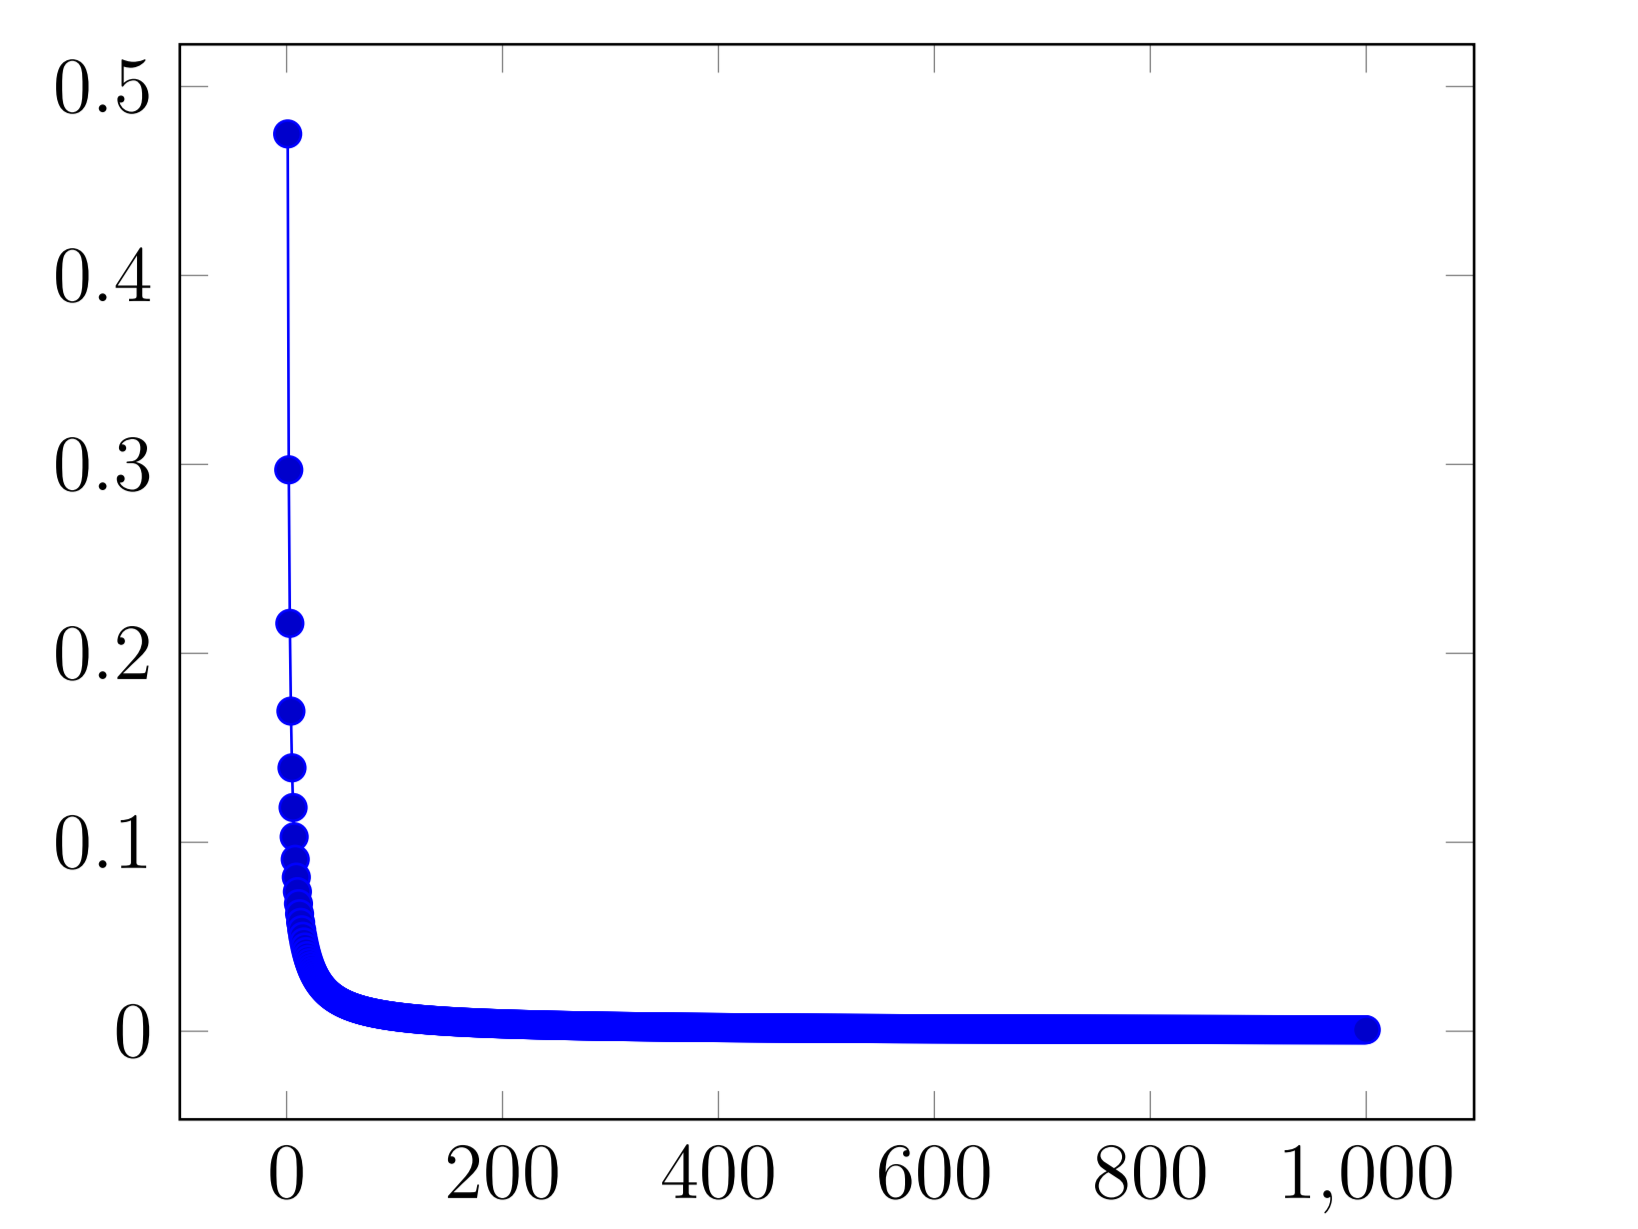
\includegraphics[scale = 0.25]{2-2.png}
        			            \caption{Разность между истинным значением числа $\pi$ и полученным нами в зависимости от номера итерации.}
        			            \label{fig:my_label}
        		          \end{figure}
                            \bigskip
                            \[\]
                            Рассмотрим промежуток от 0 до 100 итераций и посмотрим как на нём ведёт себя разность между истииным значением числа $\pi$ и полученным нами:
                            \begin{figure}[h!]
        			        \centering
        			            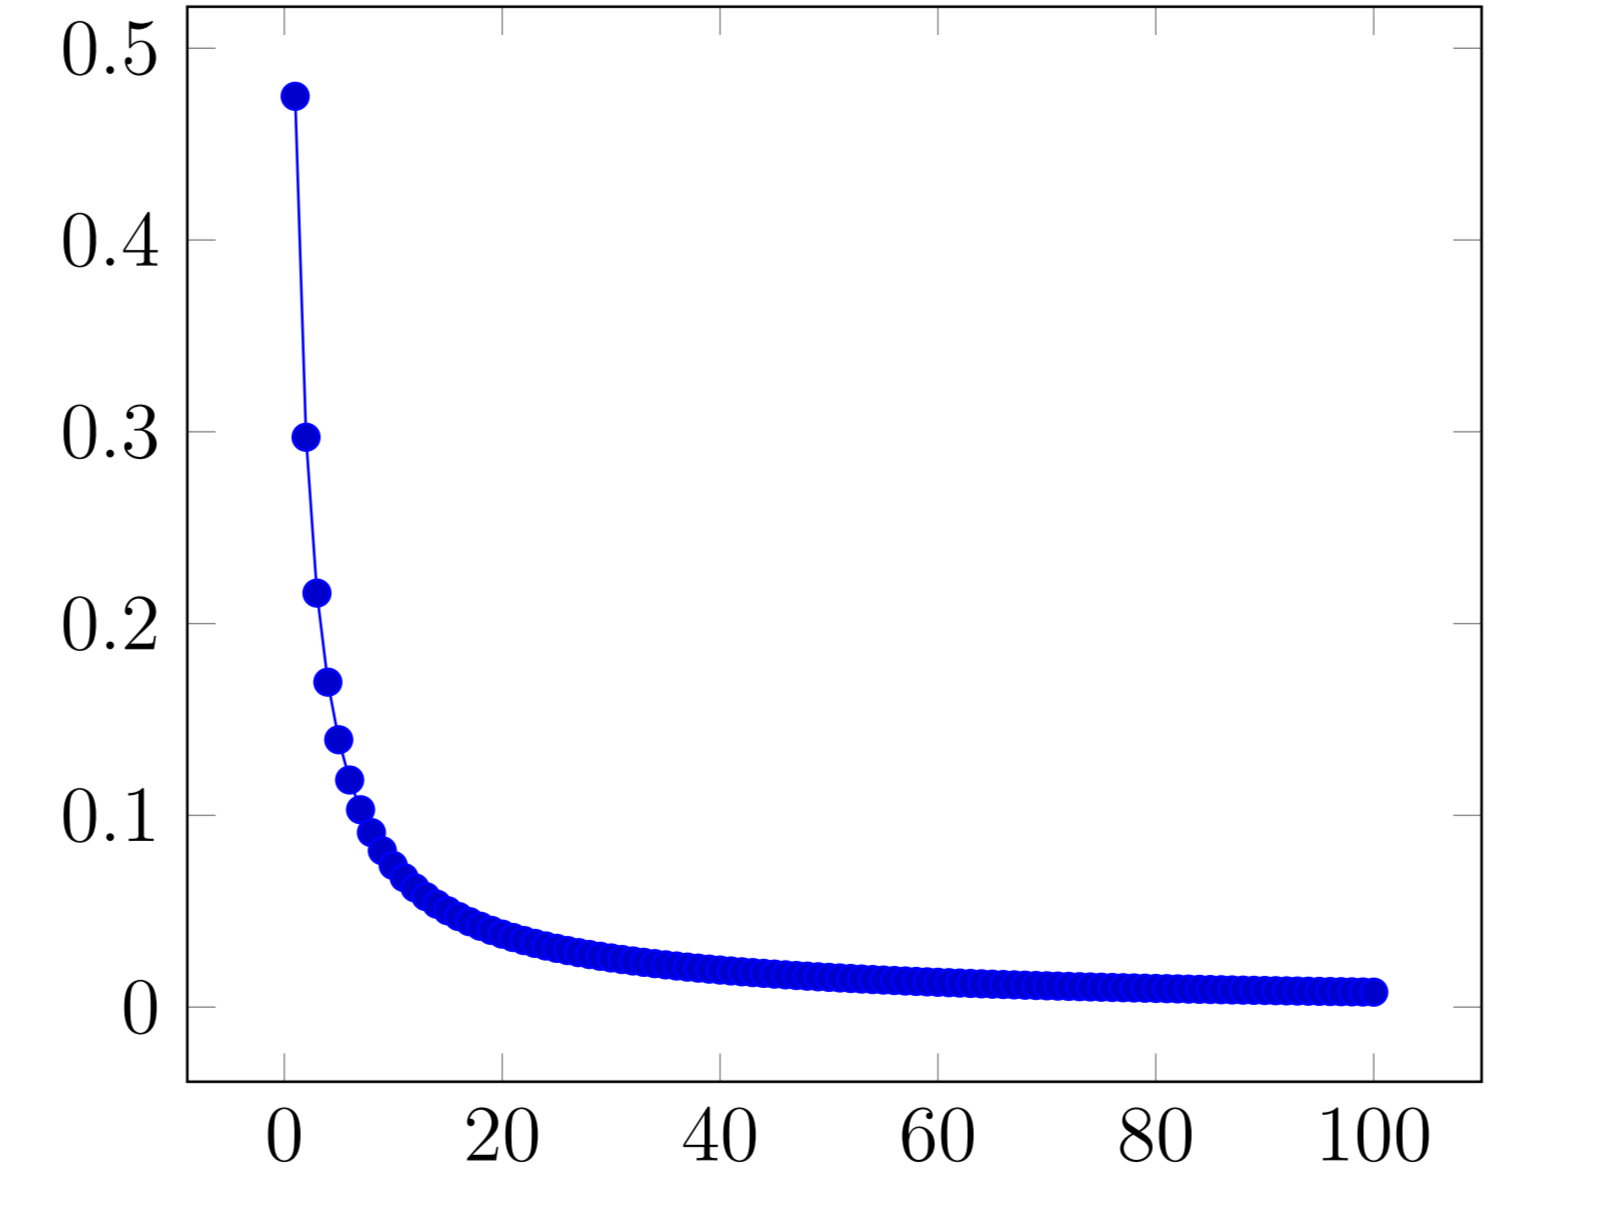
\includegraphics[scale = 0.16]{2-3.png}
        			            \caption{Разность между истинным значением числа $\pi$ и полученным нами в зависимости от номера итерации.}
        			            \label{fig:my_label}
        		          \end{figure}
                            \[\]
                            Как мы видим на графике разность стремится к нулю.
                            \newpage
                            Рассмотрим промежуток от 400 до 1000 итераций:
                            \begin{figure}[h!]
        			        \centering
        			            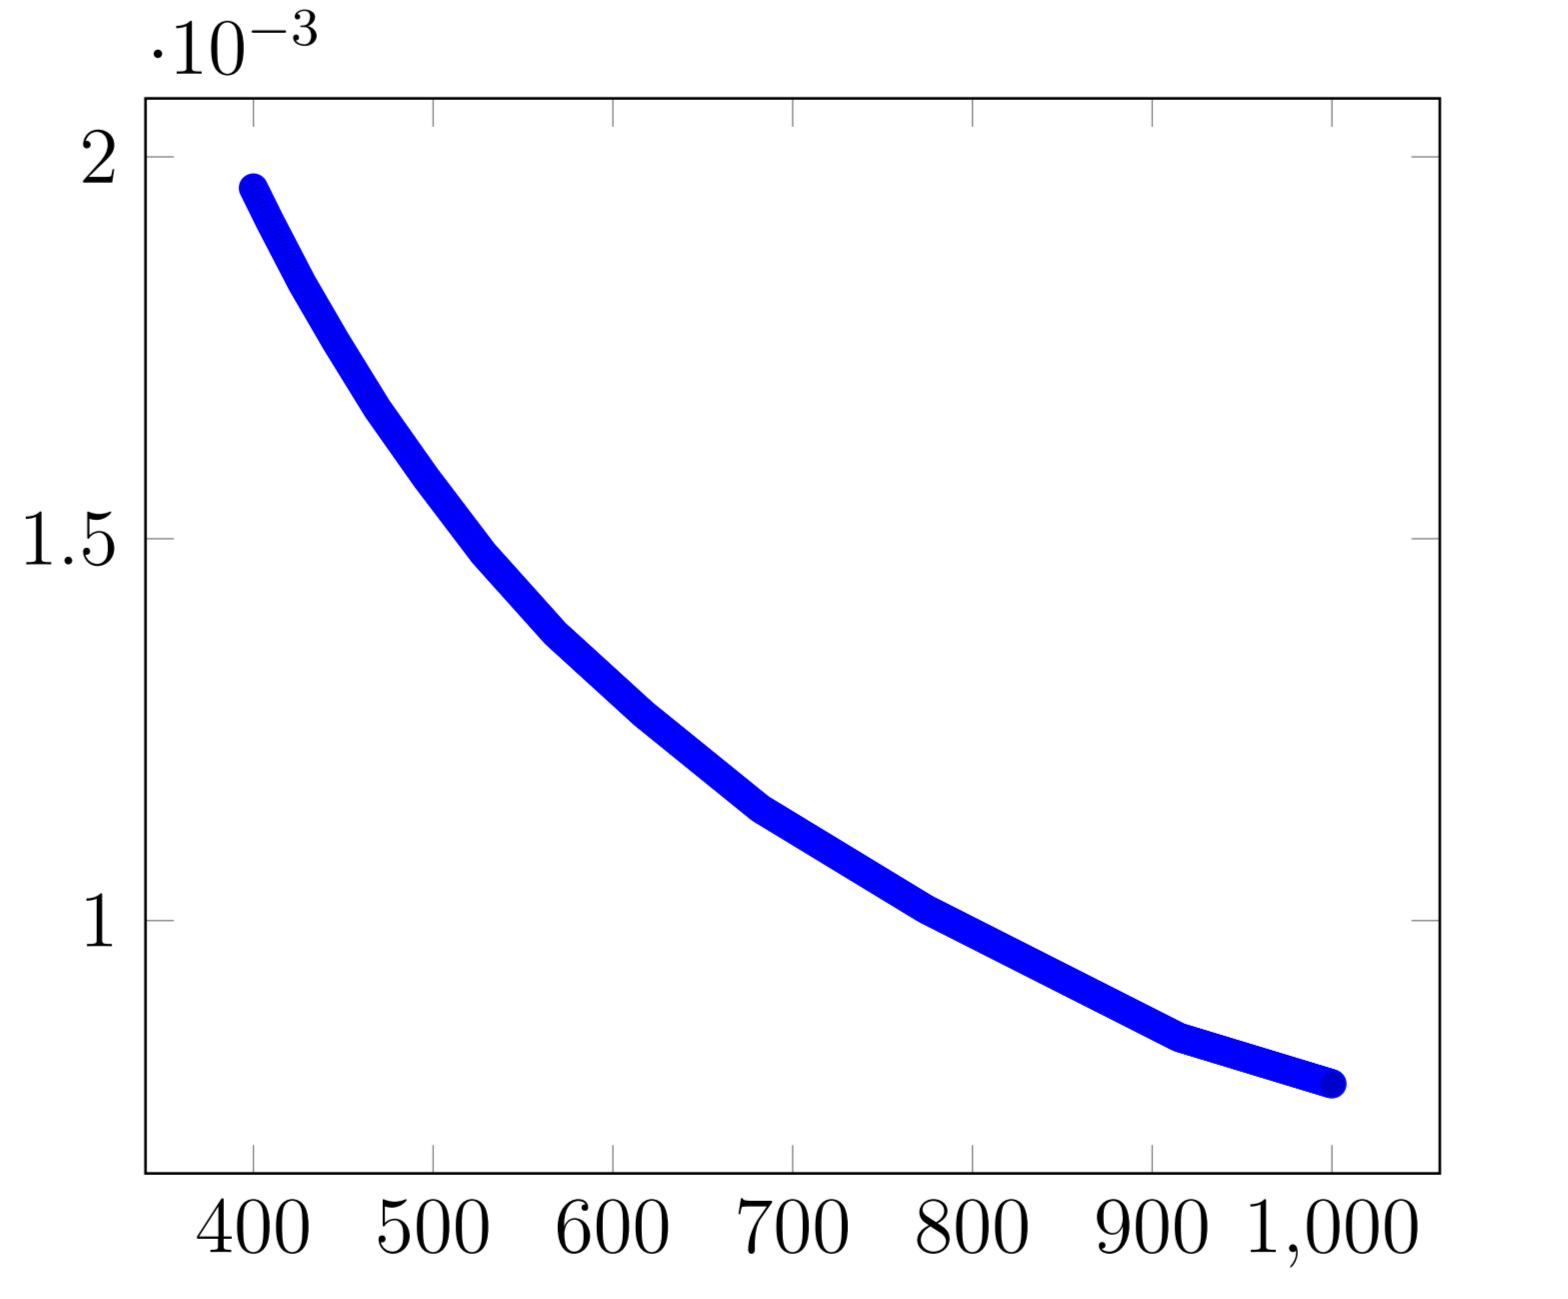
\includegraphics[scale = 0.25]{2-4.png}
        			            \caption{Разность между истинным значением числа $\pi$ и полученным нами в зависимости от номера итерации.}
        			            \label{fig:my_label}
        		          \end{figure}
                            \vskip
                            
                            Как мы видим разность стремится к нулю справа в тысячных долях.
                            \vskip
                            
                            \textbf{Следствие:} в данном случае погрешность составляет ~0.0008.
                            
                    \newpage
                    \item[\textbf{1.3: }] \textbf{Формула Виета.}
                        \begin{equation}
                            \pi = 2 \cdot \prod\limits_{i=2}^{\infty} \frac{1}{\cos{\frac{\pi}{2^i}} }
                        \end{equation}
                        \lstset { %
                            language=C++,
                            backgroundcolor=\color{black!5}, % set backgroundcolor
                            basicstyle=\footnotesize,% basic font setting
                        }
                        Используемый код:
                        \begin{lstlisting}
                #include <iostream>
                #include <math.h>
                #include <fstream>
                using namespace std;
                int main() {
                    float n, i, j;
                    float pi;
                    double PI =acos(-1.0);
                    ofstream pi_res("1.csv", ios::out);
                    while (1){
                        pi=1.0;
                        std::cout << "PI through the Viett series\n";
                        std::cout << "\nEnter the number of iterations: ";
                        std::cin >> n;
                        std::cout << "Please wait. Running..." << "\n";
                        for (i=2;i<n;i++){
                            j=1.0*pow(2,i);
                            pi *= 1/cos(PI/j);
                            pi_res << "[" << i << ", " << pi << "], ";
                        }
                    }
                    return 0;
                        
                }
                        \end{lstlisting}
                        \[\]
                        \begin{figure}[h!]
    			        \centering
    			            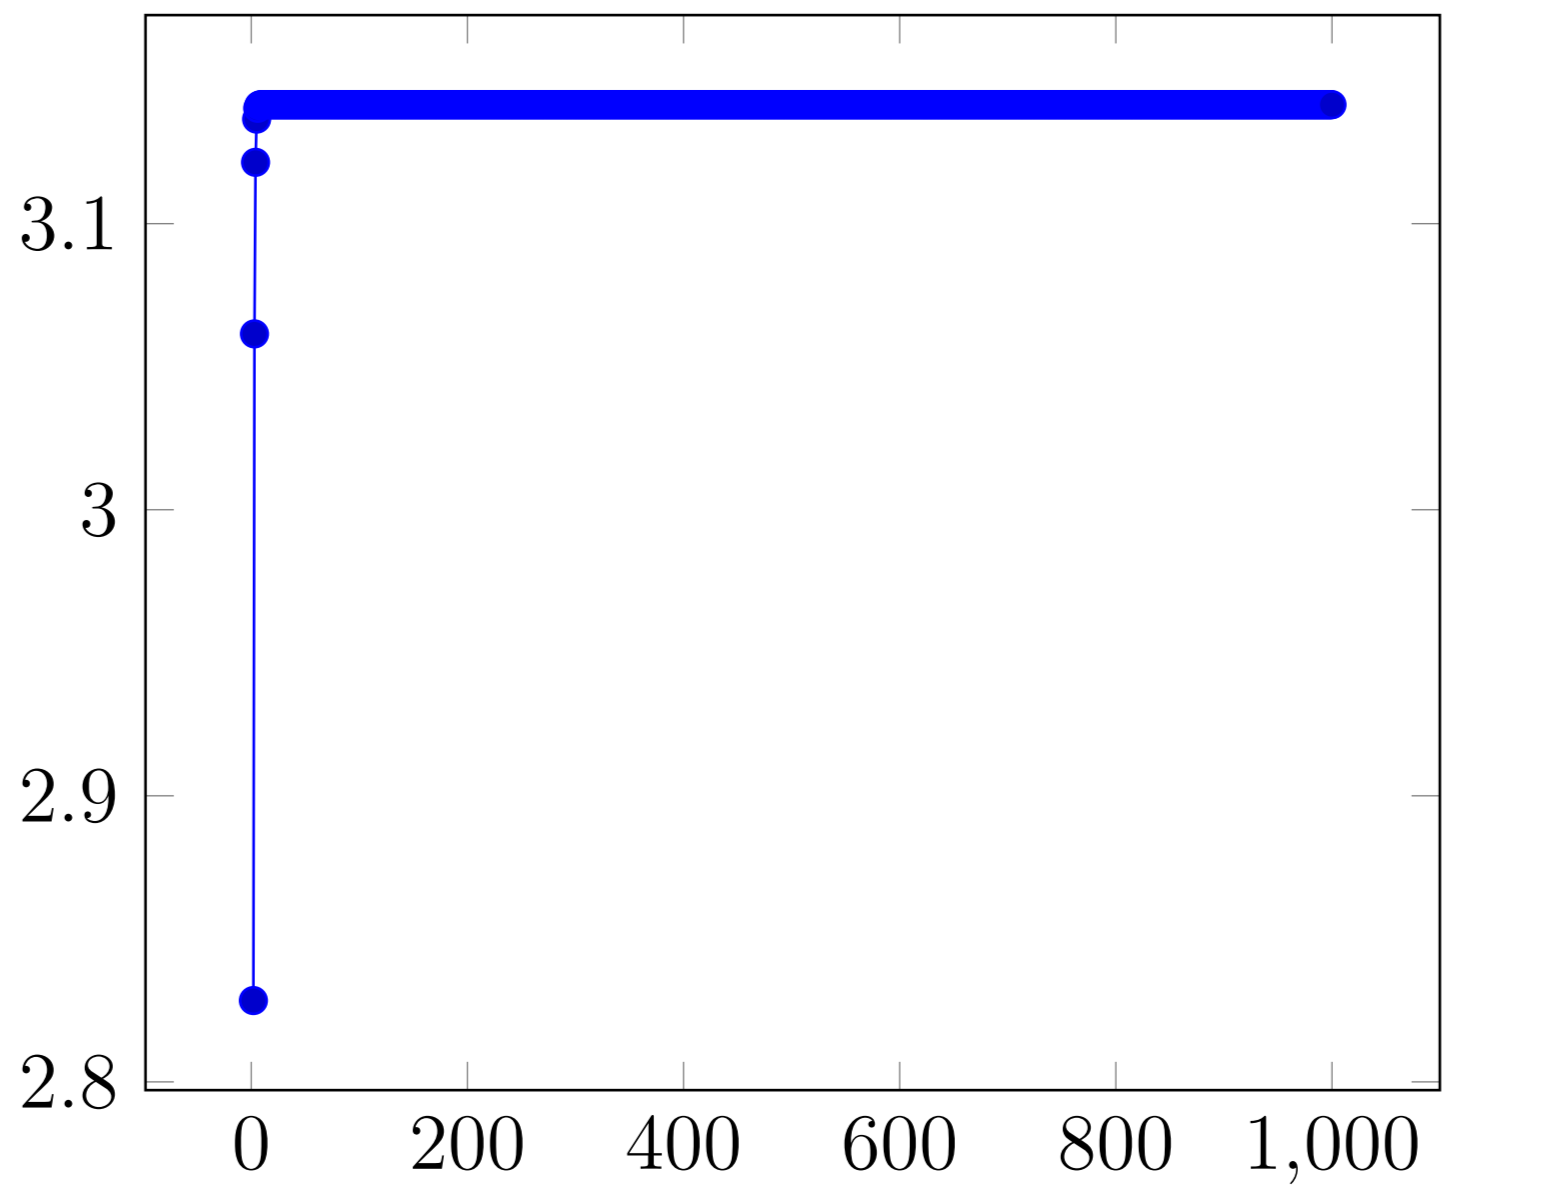
\includegraphics[scale = 0.23]{3-1.png}
    			            \caption{График зависимости числа $\pi$ от числа итераций ($n$)}
    			            \label{fig:my_label}
    		          \end{figure}
                        \newpage
                        Рассмотрим разность полученных значений с истинным в полном диапазоне итераций:
                        \begin{figure}[h!]
    			        \centering
    			            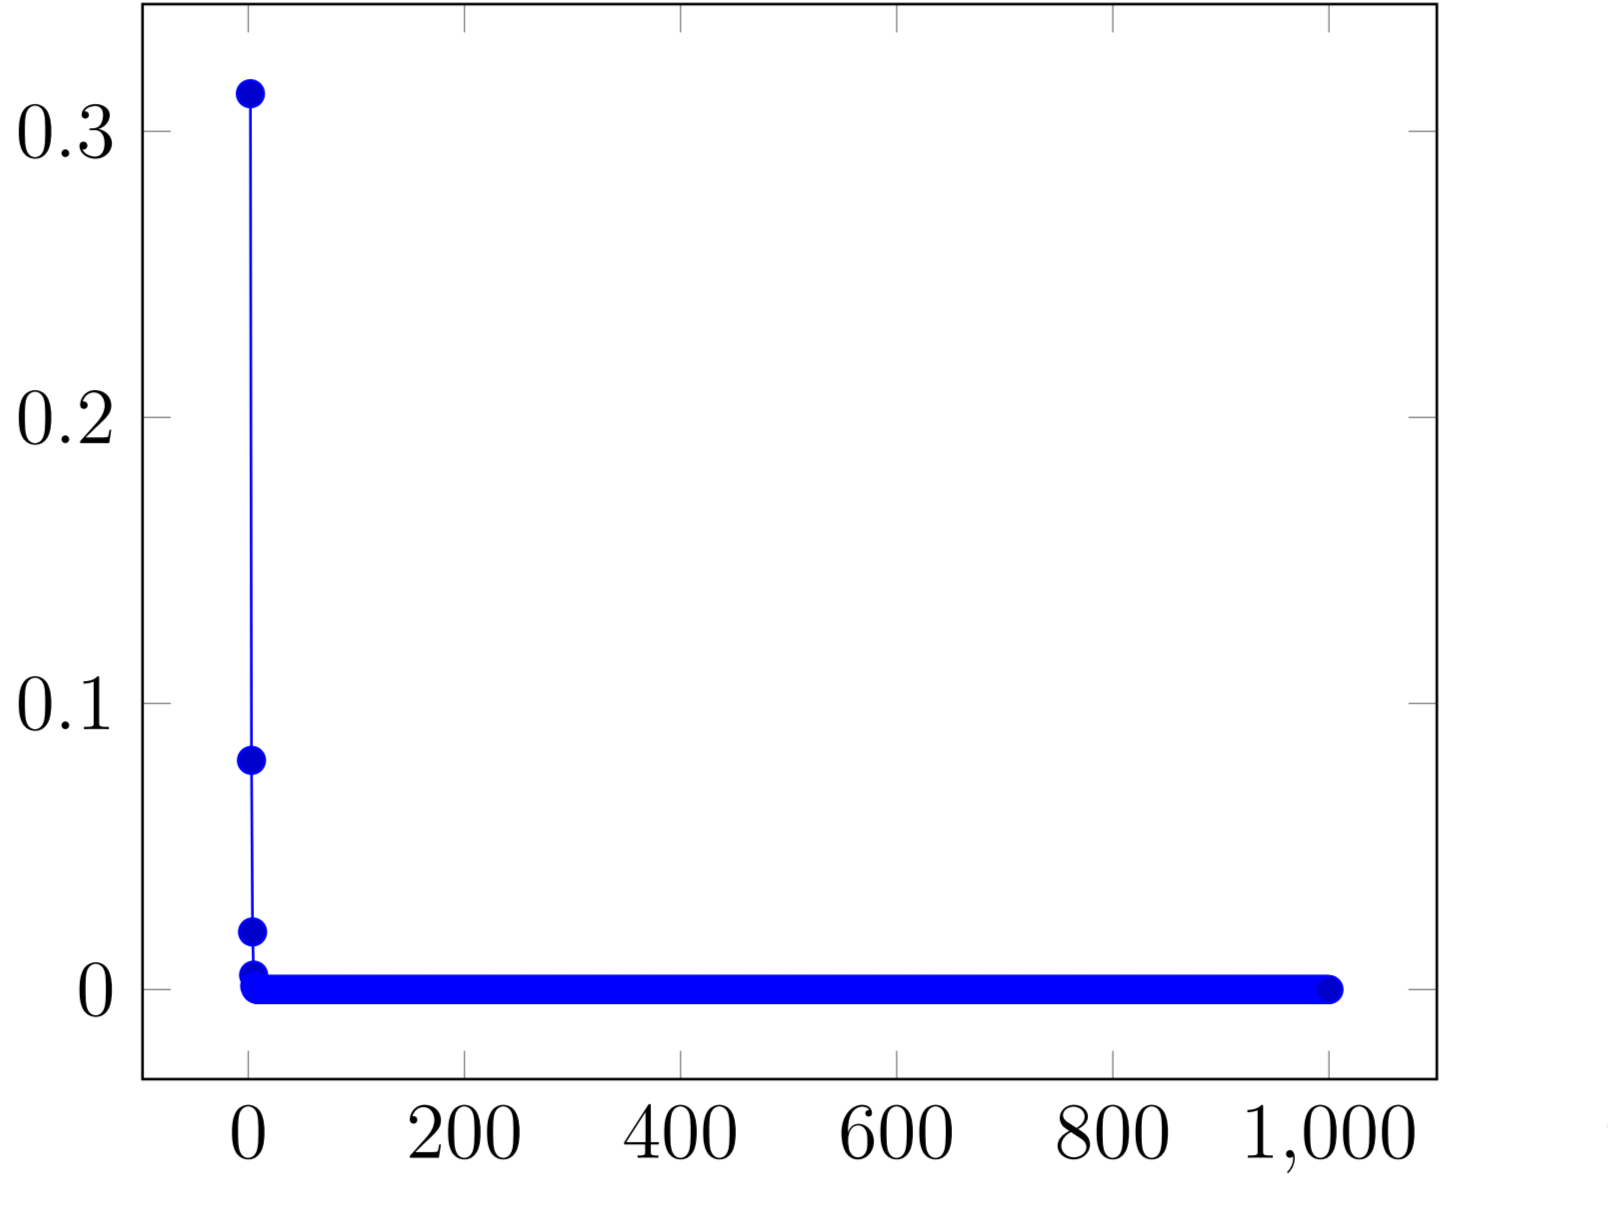
\includegraphics[scale = 0.25]{3-2.png}
    			            \caption{Разность между истинным значением числа $\pi$ и полученным нами в зависимости от номера итерации.}
    			            \label{fig:my_label}
    		          \end{figure}
                        \[\]
                        Рассмотрим поближе участок в диапазоне 2-30 итераций:
                        \begin{figure}[h!]
    			        \centering
    			            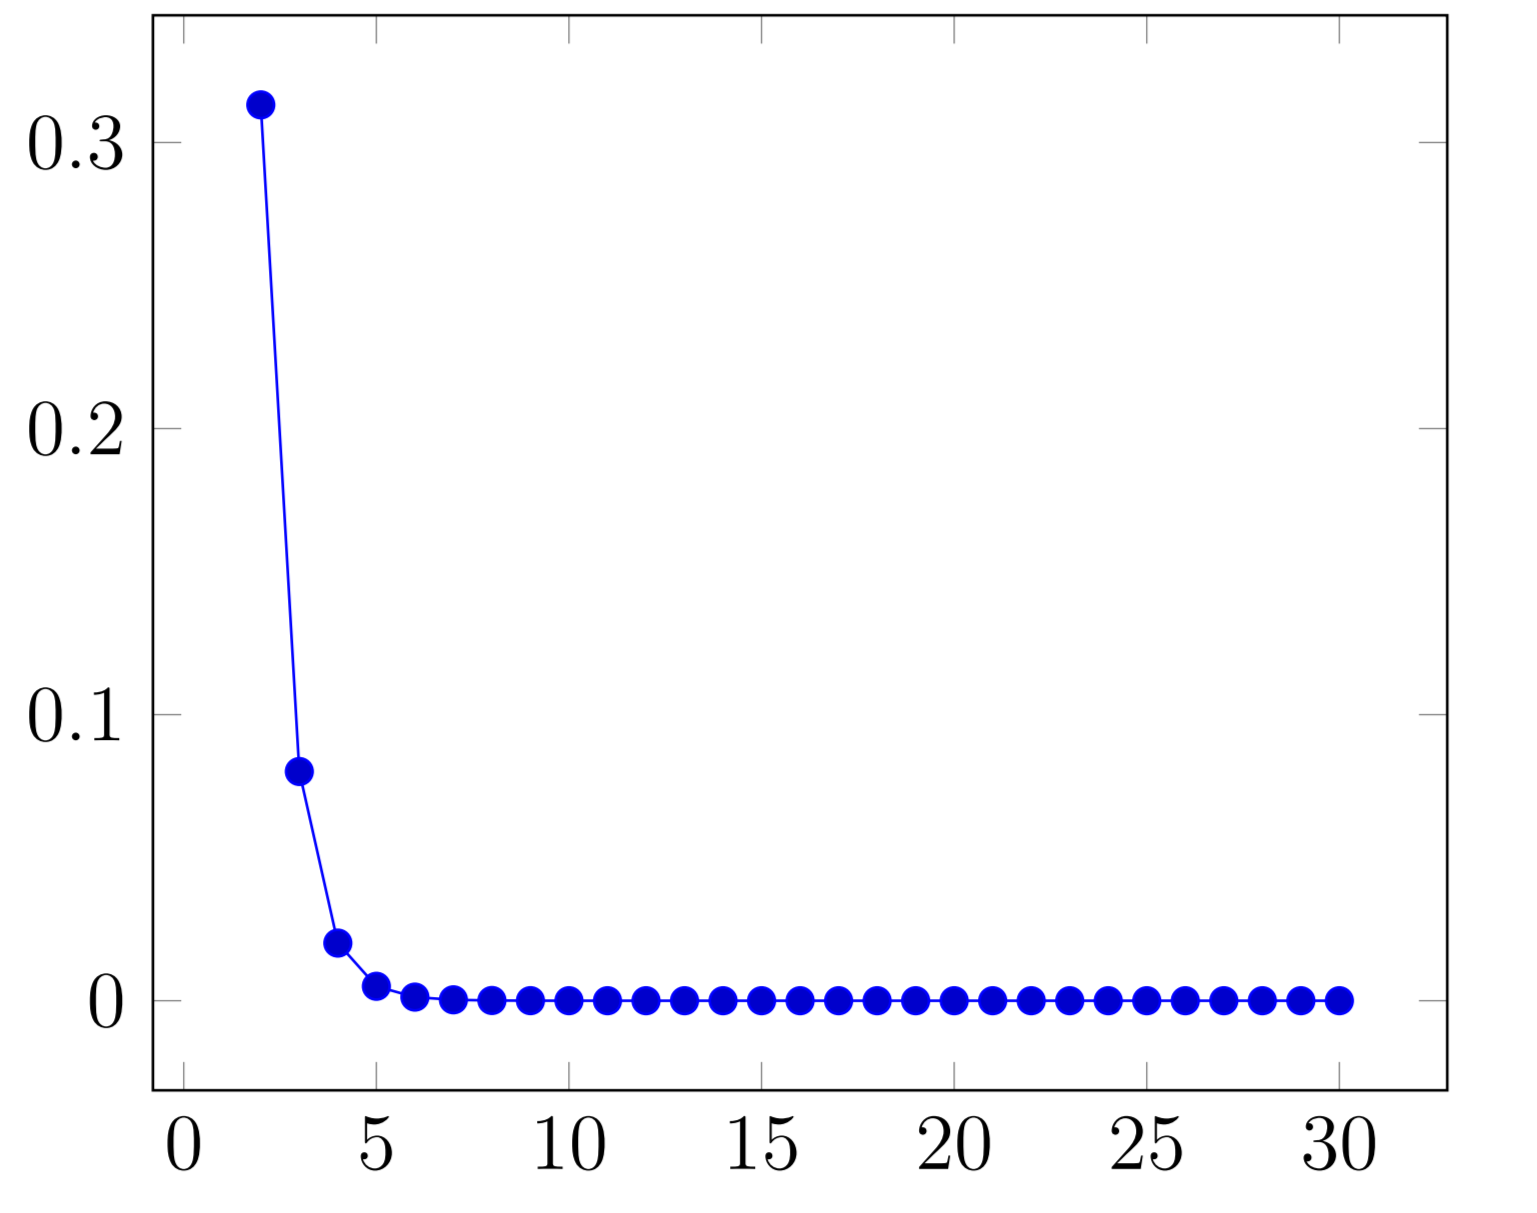
\includegraphics[scale = 0.2]{3-3.png}
    			            \caption{Разность между истинным значением числа $\pi$ и полученным нами в зависимости от номера итерации.}
    			            \label{fig:my_label}
    		          \end{figure}
                        \newpage
                        А теперь рассмотрим участок от 700 итерации до 1000-ной:
                        \begin{figure}[h!]
    			        \centering
    			            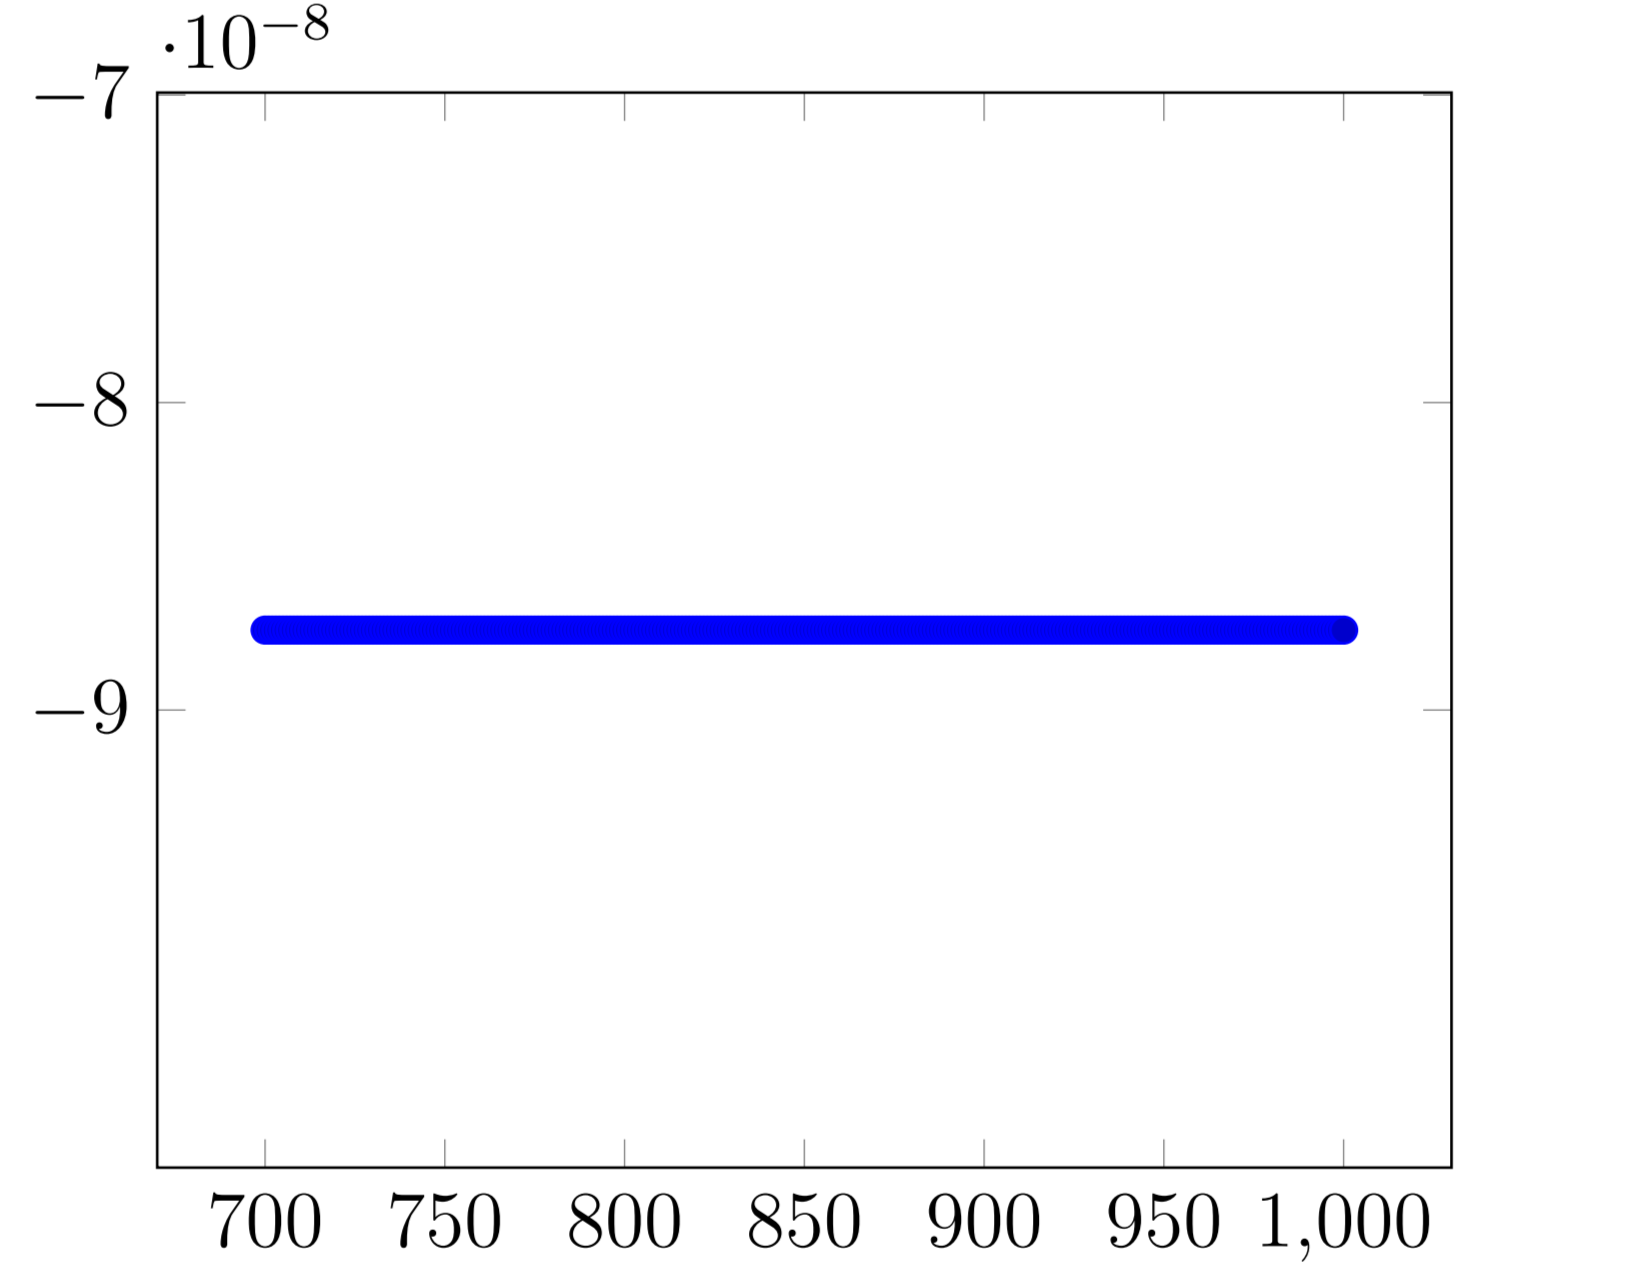
\includegraphics[scale = 0.2]{3-4.png}
    			            \caption{Разность между истинным значением числа $\pi$ и полученным нами в зависимости от номера итерации.}
    			            \label{fig:my_label}
    		          \end{figure}
                        \vskip
                        
                        Заметим странную вещь: по графику видно, что начиная с некоторого элемента значения числа $\pi$, полученного нами, не меняются. Разберёмся - это ошибка вычислений, баг или особенность формулы?
                        Рассмотрим некоторый элемент с индексом $i$: 
                        \[
                            a_{i}=\lim\limits_{i \rightarrow {\infty}} \cos{\frac{\pi}{2^i}} = \cos{\lim\limits_{i \rightarrow {\infty}} \frac{\pi}{2^i}} = \cos{0} = 1
                        \]
                        А как известно при домножении на 1 числа не меняются, эт этого наше значение $\pi$ и не меняется. Вывод - это не ошибка, а особенность формулы, которую мы использовали для вычислений.
                        \vskip
                        
                        \textbf{Следствие:} При 1000 сомножителях точность достигает $1 \cdot 10^7$
                                        
                    \newpage
                    \item[1.4: ] \textbf{Преобразование Мандхава.}
                        \begin{equation}
                            \pi = 2\sqrt{3} \cdot \sum\limits_{i=0}^{\infty} \frac{(-1)^i}{3^i \cdot (2i+1)}
                        \end{equation}
                        \vskip
                        
                        \lstset { %
                            language=C++,
                            backgroundcolor=\color{black!5}, % set backgroundcolor
                            basicstyle=\footnotesize,% basic font setting
                            }
                        Используемый код:
                        \begin{lstlisting}            
                #include <iostream>
                #include <math.h>
                #include <fstream>
                using namespace std;
                int main() {
                    float n, i, j;
                    float pi;
                    double PI =acos(-1.0);
                    ofstream pi_res("1.csv", ios::out);
                    while (1){
                        pi=0.0;
                        std::cout << "PI through the Mandha's series\n";
                        std::cout << "\nEnter the number of iterations: ";
                        std::cin >> n;
                        std::cout << "Please wait. Running..." << "\n";
                        for (i=0;i<n;i++){
                            if (i%2==0) j=2*sqrt(3)/(pow(3,i)*(2*i+1));
                            else j=(2*sqrt(3)/(pow(3,i)*(2*i+1)))*(-1);
                            pi+=j;
                            pi_res << "[" << i << ", " << pi << "], ";
                    }
                   return 0;
                }  
                        \end{lstlisting}
                        \bigskip
                        \begin{figure}[h!]
        		        \centering
    		              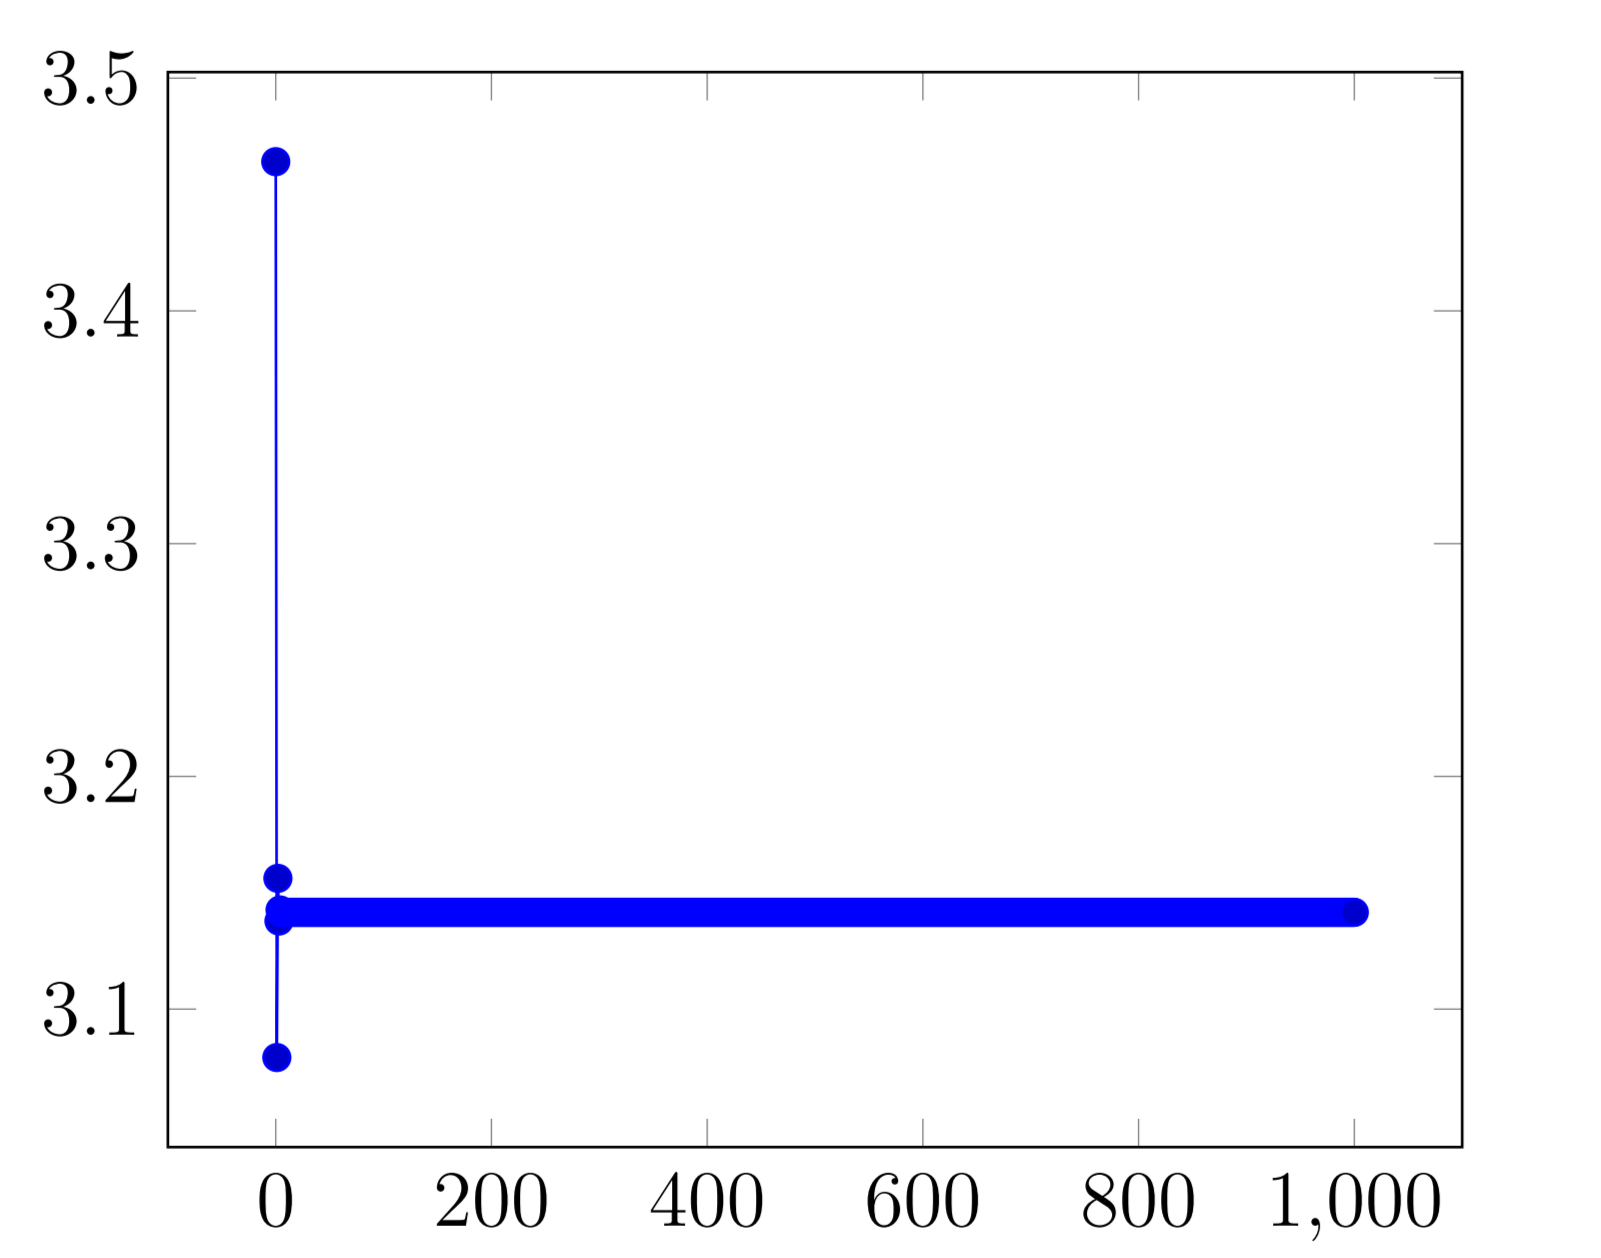
\includegraphics[scale = 0.22]{4-1.png}
    		              \caption{График зависимости числа $\pi$ от числа итераций ($n$)}
                            \label{fig:my_label}
        		        \end{figure}
                        \newpage
                        Разность с истинным значением $\pi$ для всех итераций на графике: 
                        \begin{figure}[h!]
        		        \centering
    		              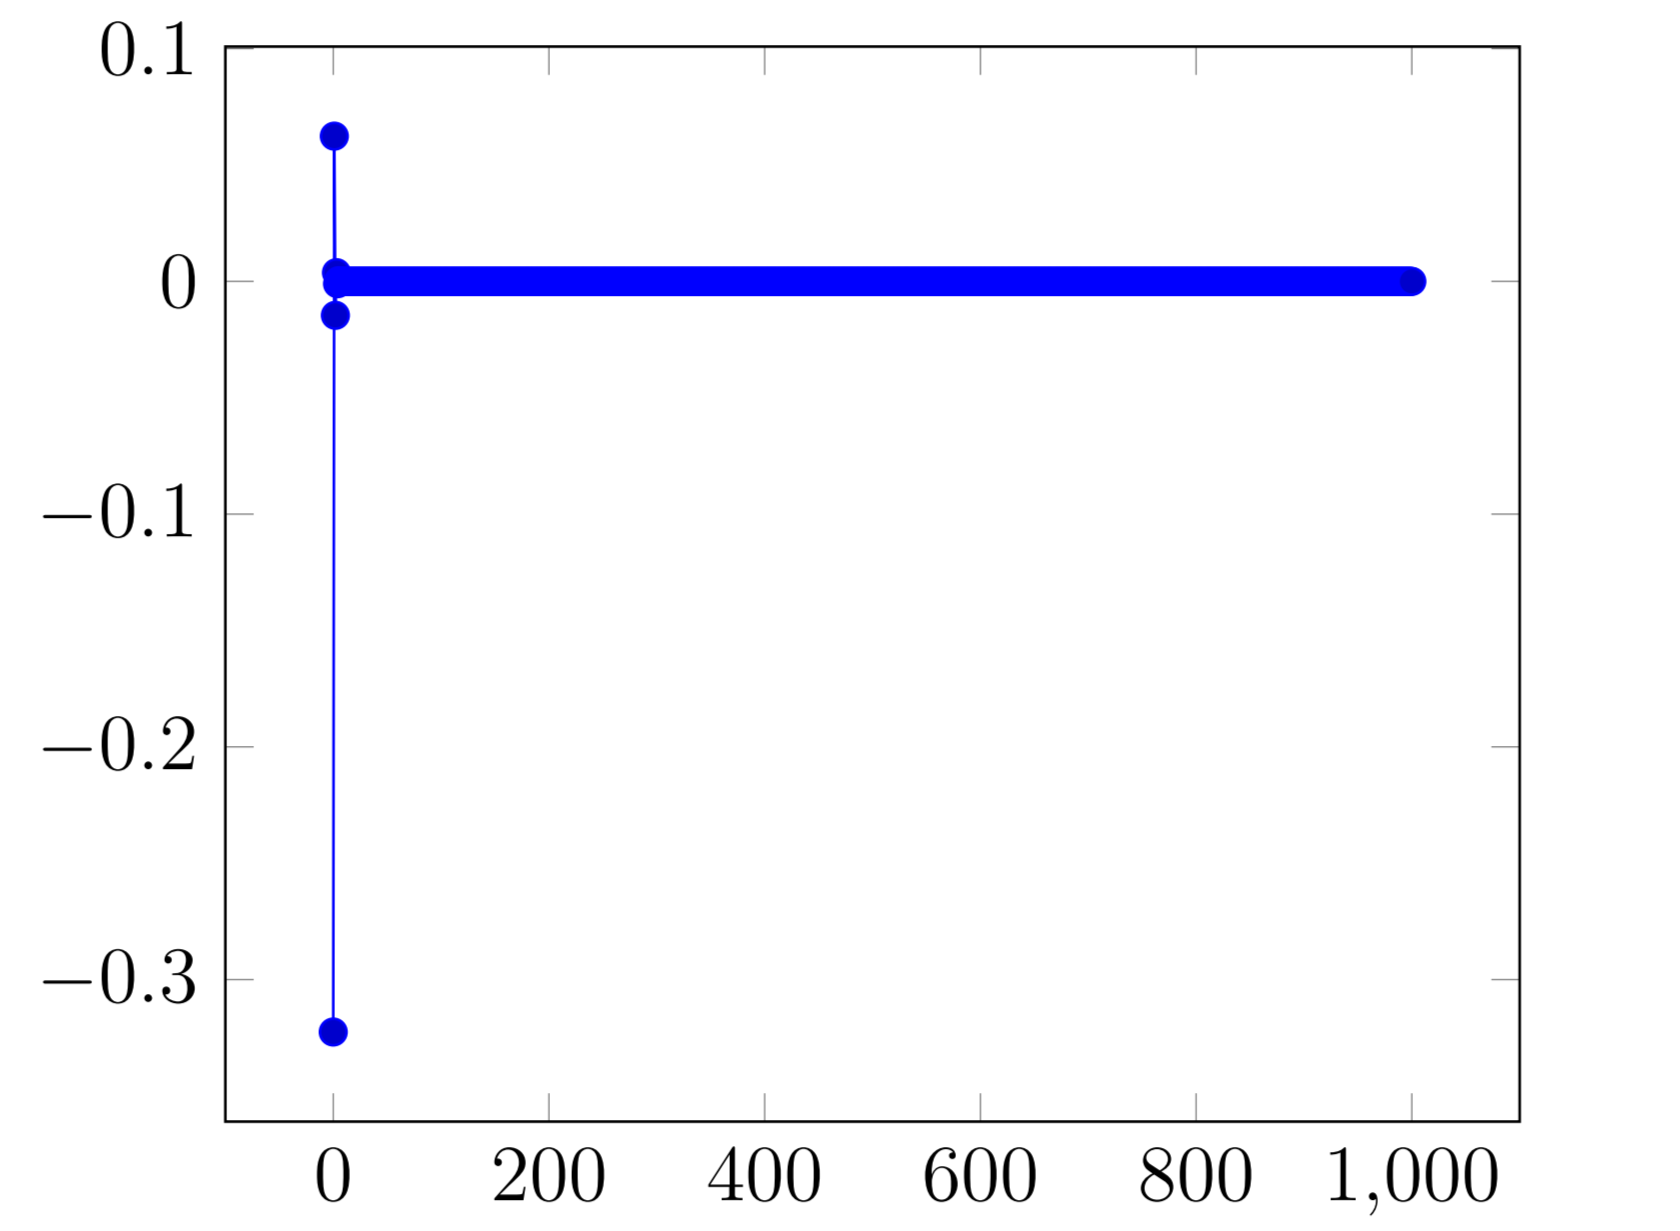
\includegraphics[scale = 0.2]{4-2.png}
    		              \caption{Разность с истинным значнием в зависимости от числа итераций ($n$)}
                            \label{fig:my_label}
        		        \end{figure}
                        \[\]
                        Как мы видим, опять значения в какой-то момент перестают меняться. Рассмотрим малый промежуток, число итераций меньше 30:
                        \begin{figure}[h!]
        		        \centering
    		              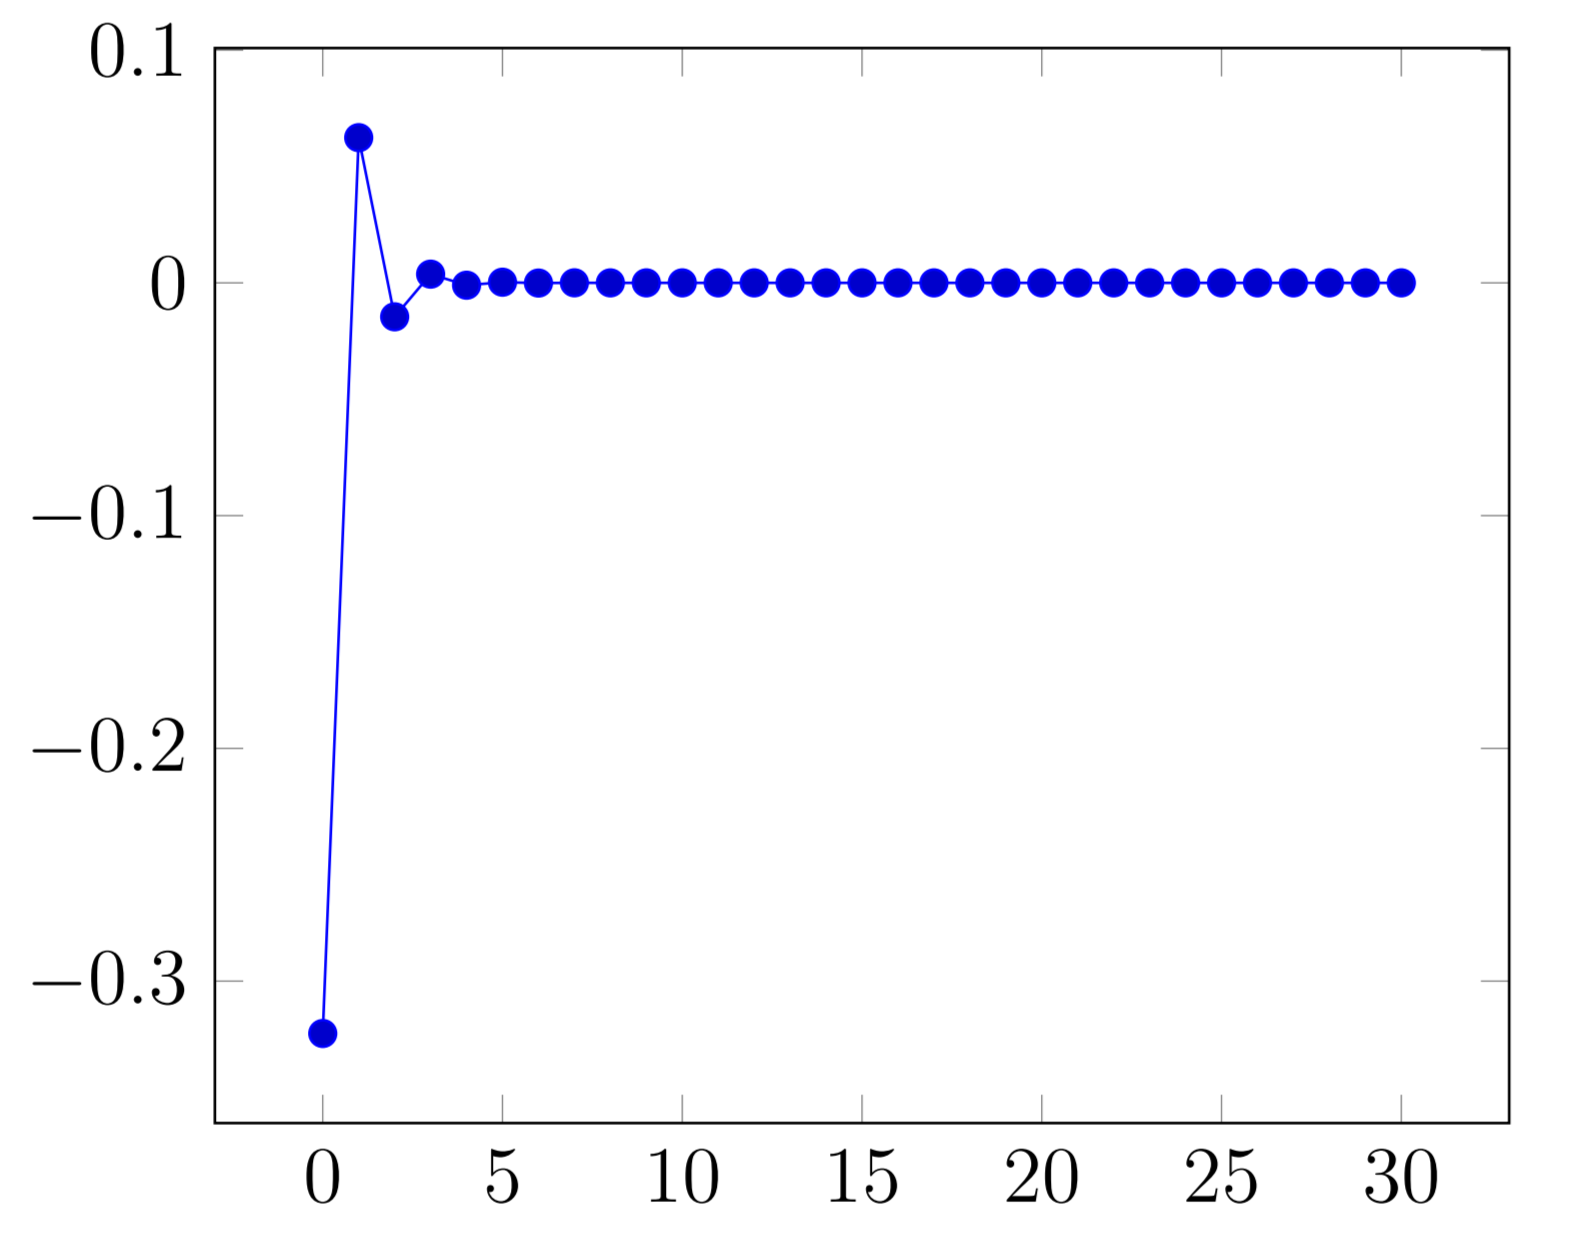
\includegraphics[scale = 0.2]{4-3.png}
    		              \caption{Разность с истинным значнием в зависимости от числа итераций ($n$)}
                            \label{fig:my_label}
        		        \end{figure}
                        \newpage
                        Теперь рассмотрим большое число итераций, ведь опять начиная с некоторого слагаемого сумма не меняется:
                        \[
                        a_{i} = \lim\limits_{i \rightarrow \infty} \frac{(-1)^i}{3^i \cdot (2i+1)} = 0 
                        \Longrightarrow a_{i} \rightarrow 0
                        \]
                        Это значит, что начиная с некоторой итерации $a_{i}$ будет равно 0, следовательно сумма перестанет меняться.
                        \vskip
                        \textbf{Следовательно:} Для данного способа нахождения $\pi$ погрешность измерения составляет около $1*10^{-6}$. (для итераций $\rightarrow$ 1000)
                \end{enumerate}
            \vskip
            \item \textbf{Задание 5:} Рассчет времени обработки.
            Рассчитаем время используя стандартную функцию для измерения времени:
                \lstset { %
                language=C++,
                backgroundcolor=\color{black!5}, % set backgroundcolor
                basicstyle=\footnotesize,% basic font setting
                }
                Используемый фрагмент кода:
                \begin{lstlisting}
            #include <chrono>
            double get_time() {
            return std::chrono::duration_cast<std::chrono::microseconds>
            (std::chrono::steady_clock::now().time_since_epoch()).count()/1e6;
            }       
                \end{lstlisting}
                \[\]
                По полученным данным составим графики зависимости. Для каждой формулы, описанной выше, оценим время, за которая эта формула доходит до 10 знака после запятой в числе $\pi$.
                \[\]
                \textbf{Время для формулы Лейбница:}
                \begin{figure}[h!]
        		\centering
                    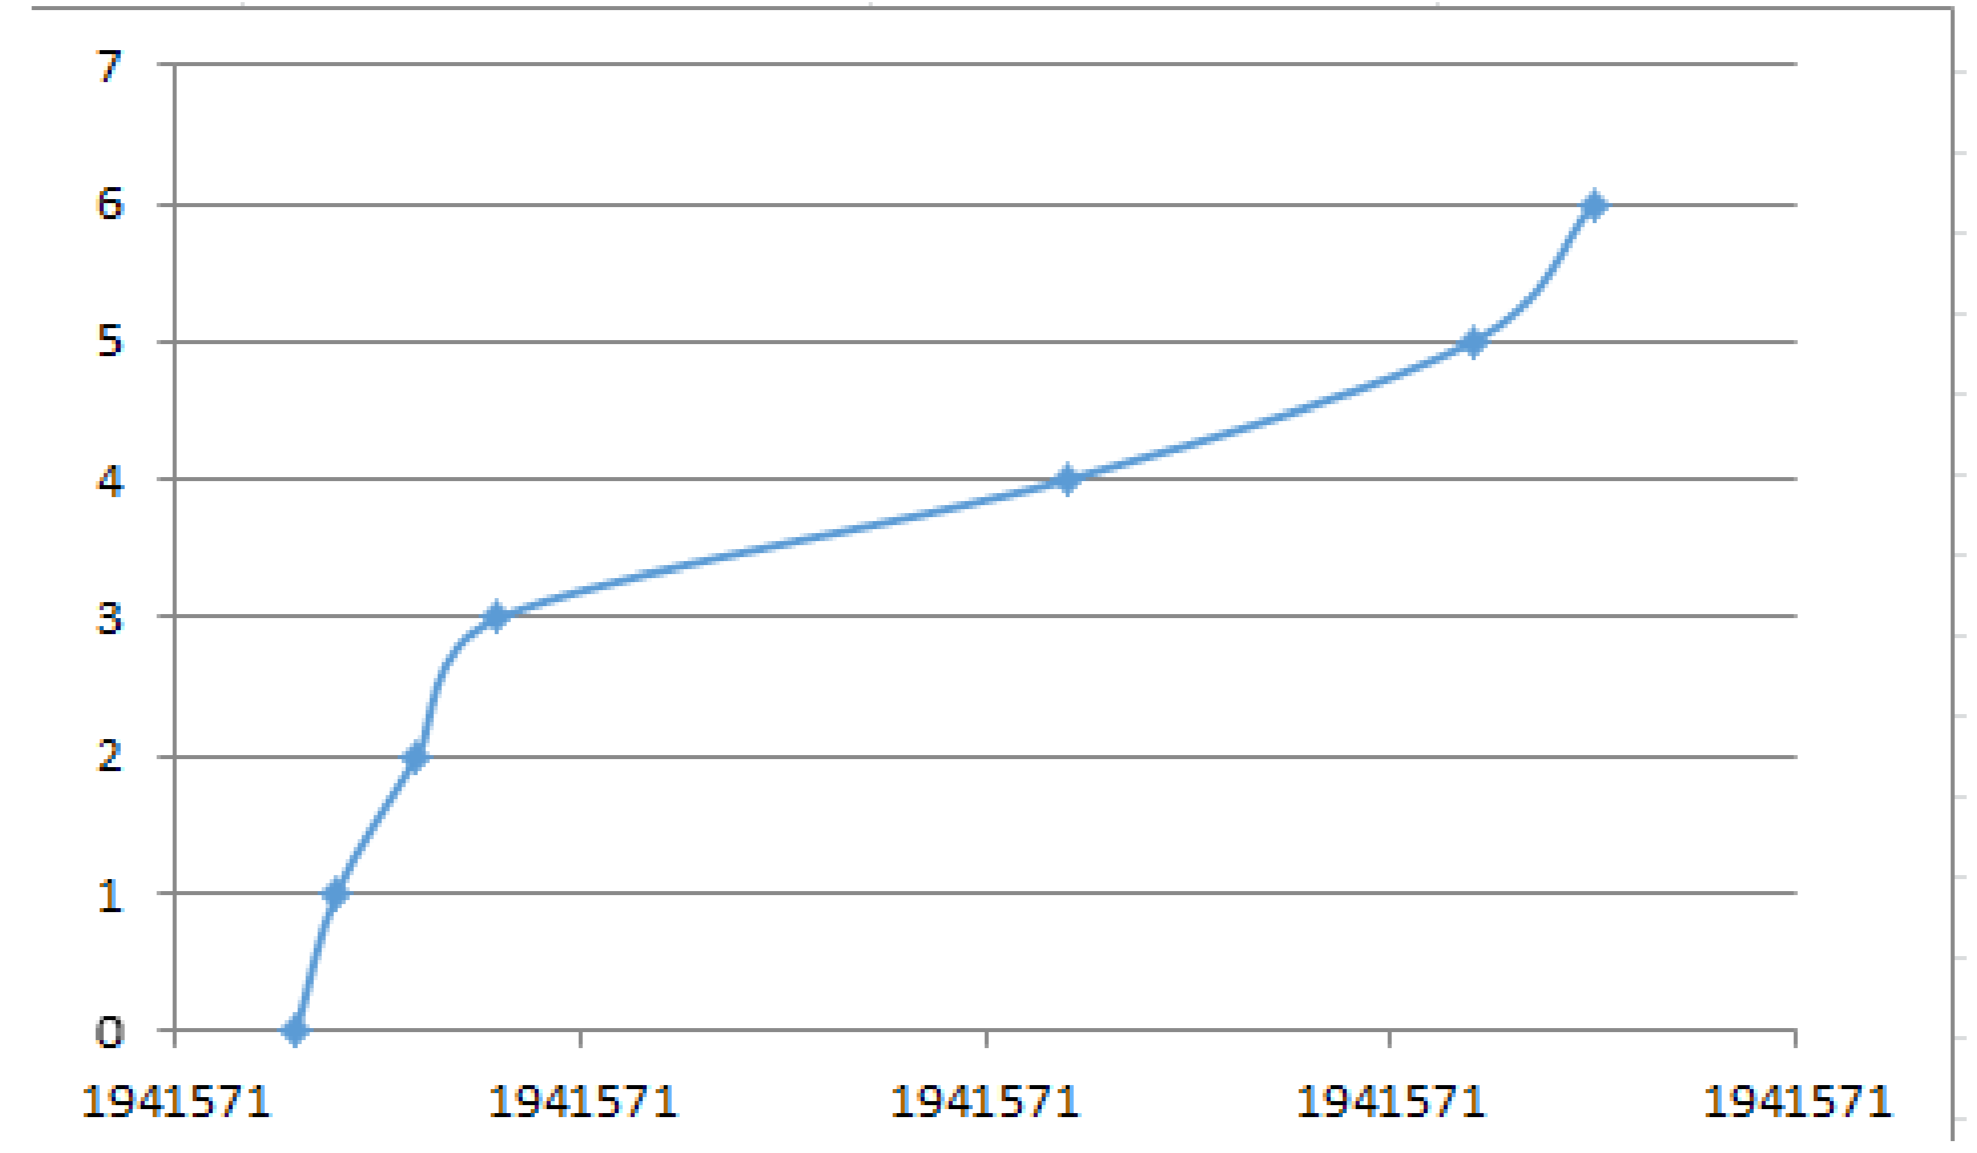
\includegraphics[scale = 0.25]{5-1.png}
	              \caption{Время рассчёта 10 знакп после запятой в числе $\pi$}
                    \label{fig:my_label}
	        \end{figure}
                \newpage
                \textbf{Время для формулы Валлиса:}
                \begin{figure}[h!]
    	        \centering
    	        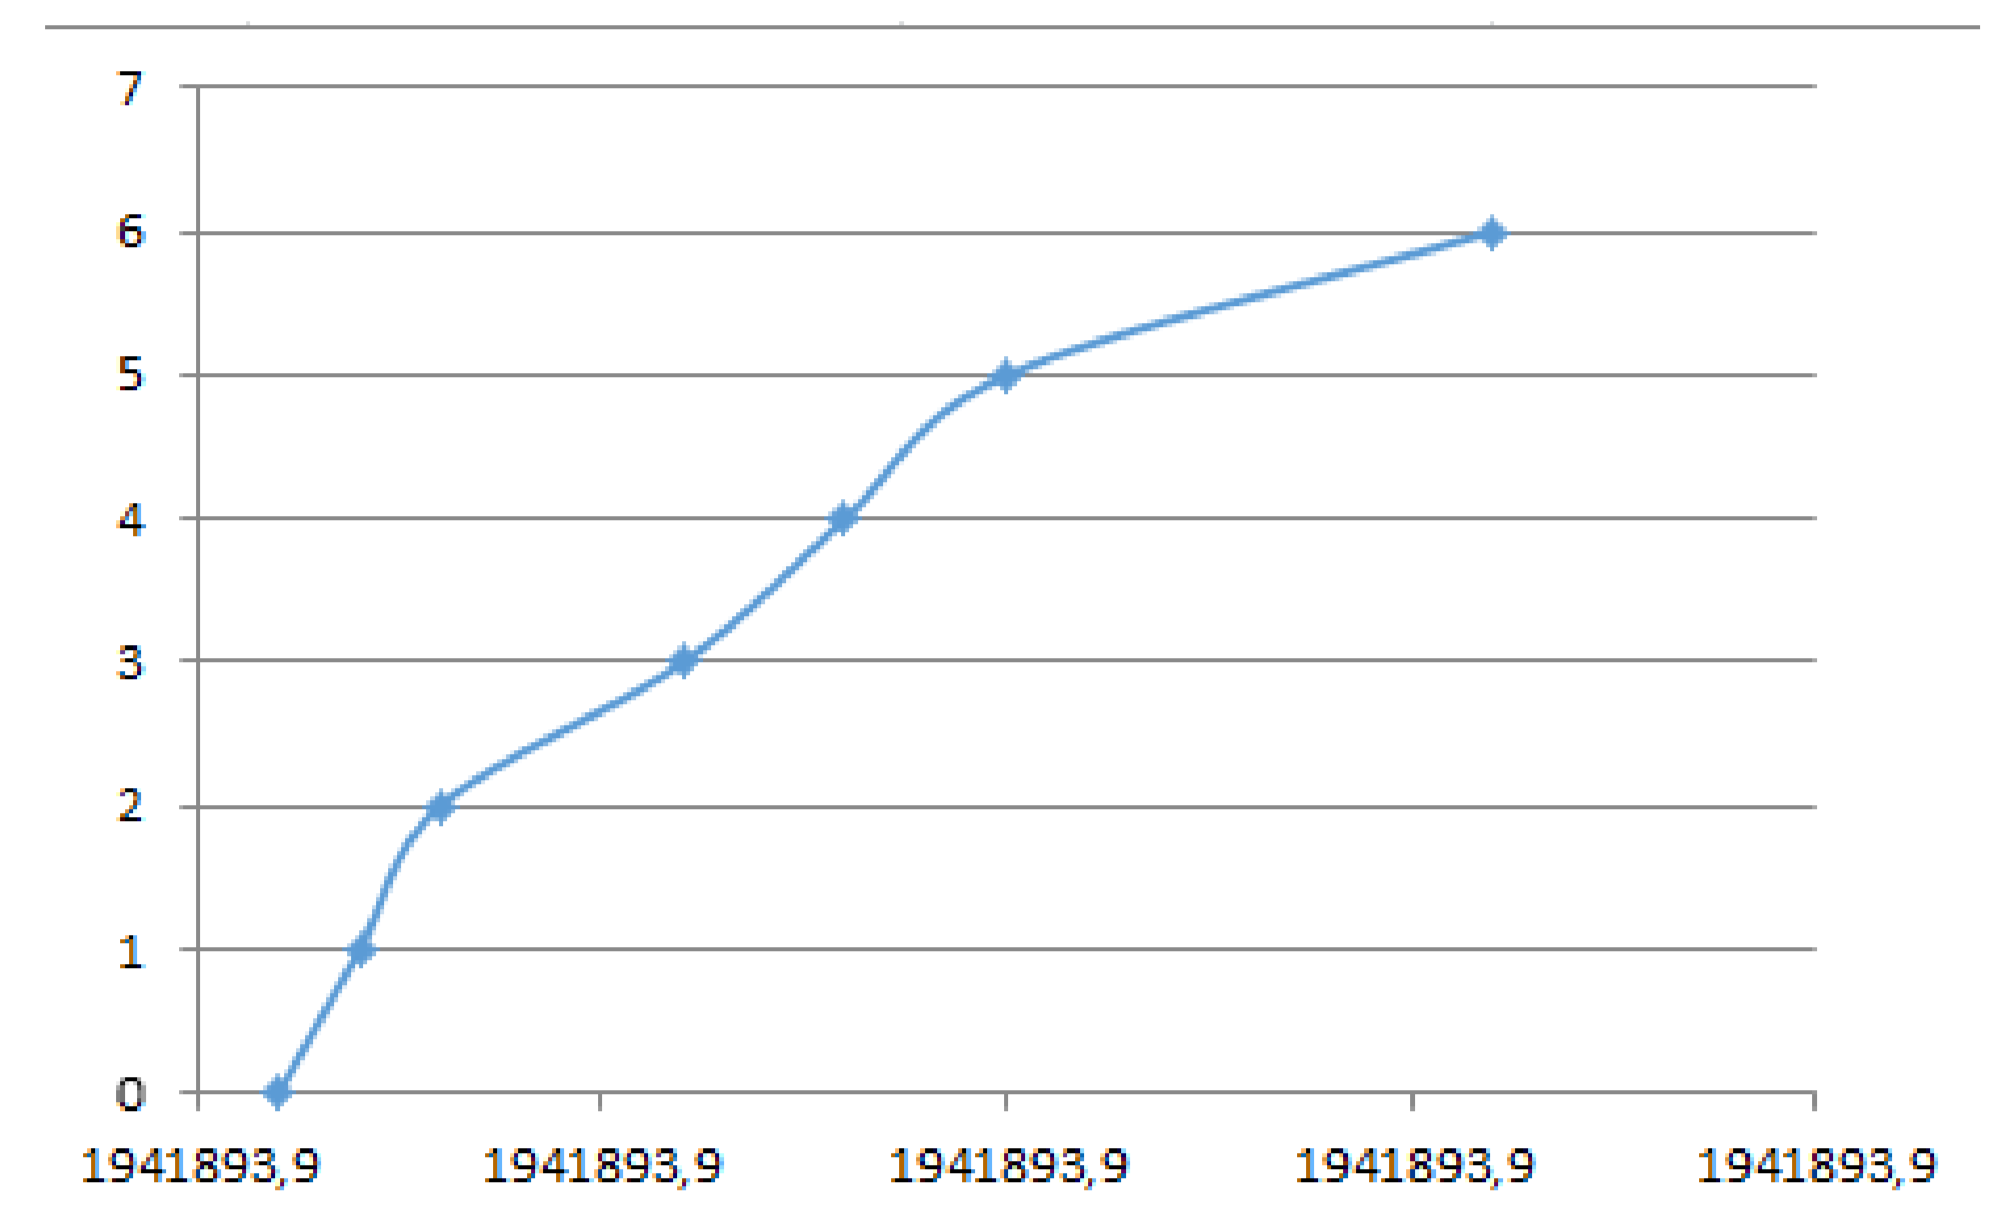
\includegraphics[scale = 0.25]{5-2.png}
    		    \caption{Время рассчёта 10 знакп после запятой в числе $\pi$}
                    \label{fig:my_label}
        		\end{figure}
          \[\]
                \textbf{Время для формулы Виетта:}
                \begin{figure}[h!]
    	        \centering
    	        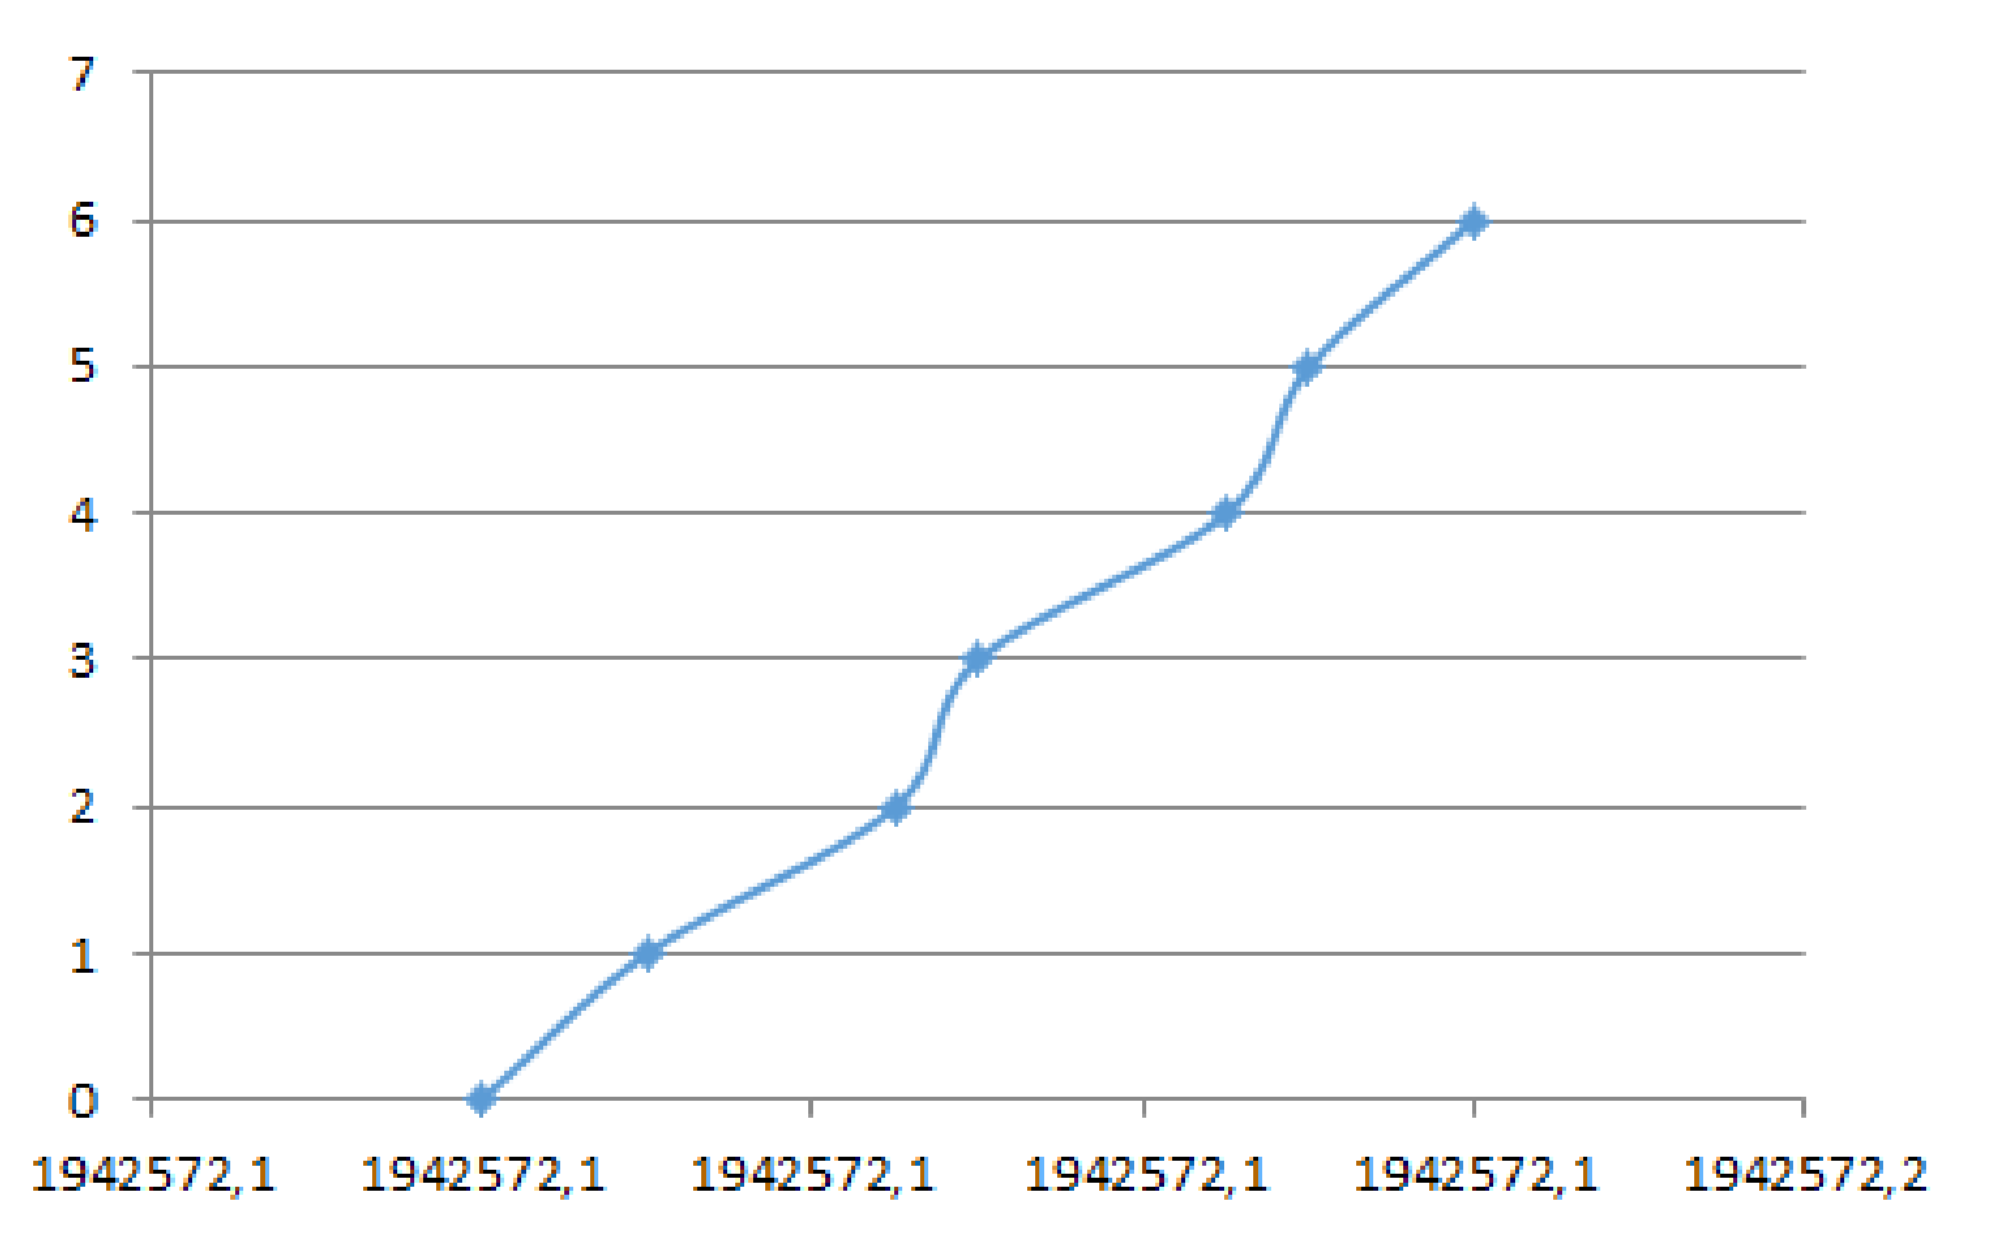
\includegraphics[scale = 0.25]{5-3.png}
    		    \caption{Время рассчёта 10 знакп после запятой в числе $\pi$}
                    \label{fig:my_label}
        		\end{figure}
                \newpage
                \textbf{Время для формулы Мандхава:}
                \begin{figure}[h!]
    	        \centering
    	        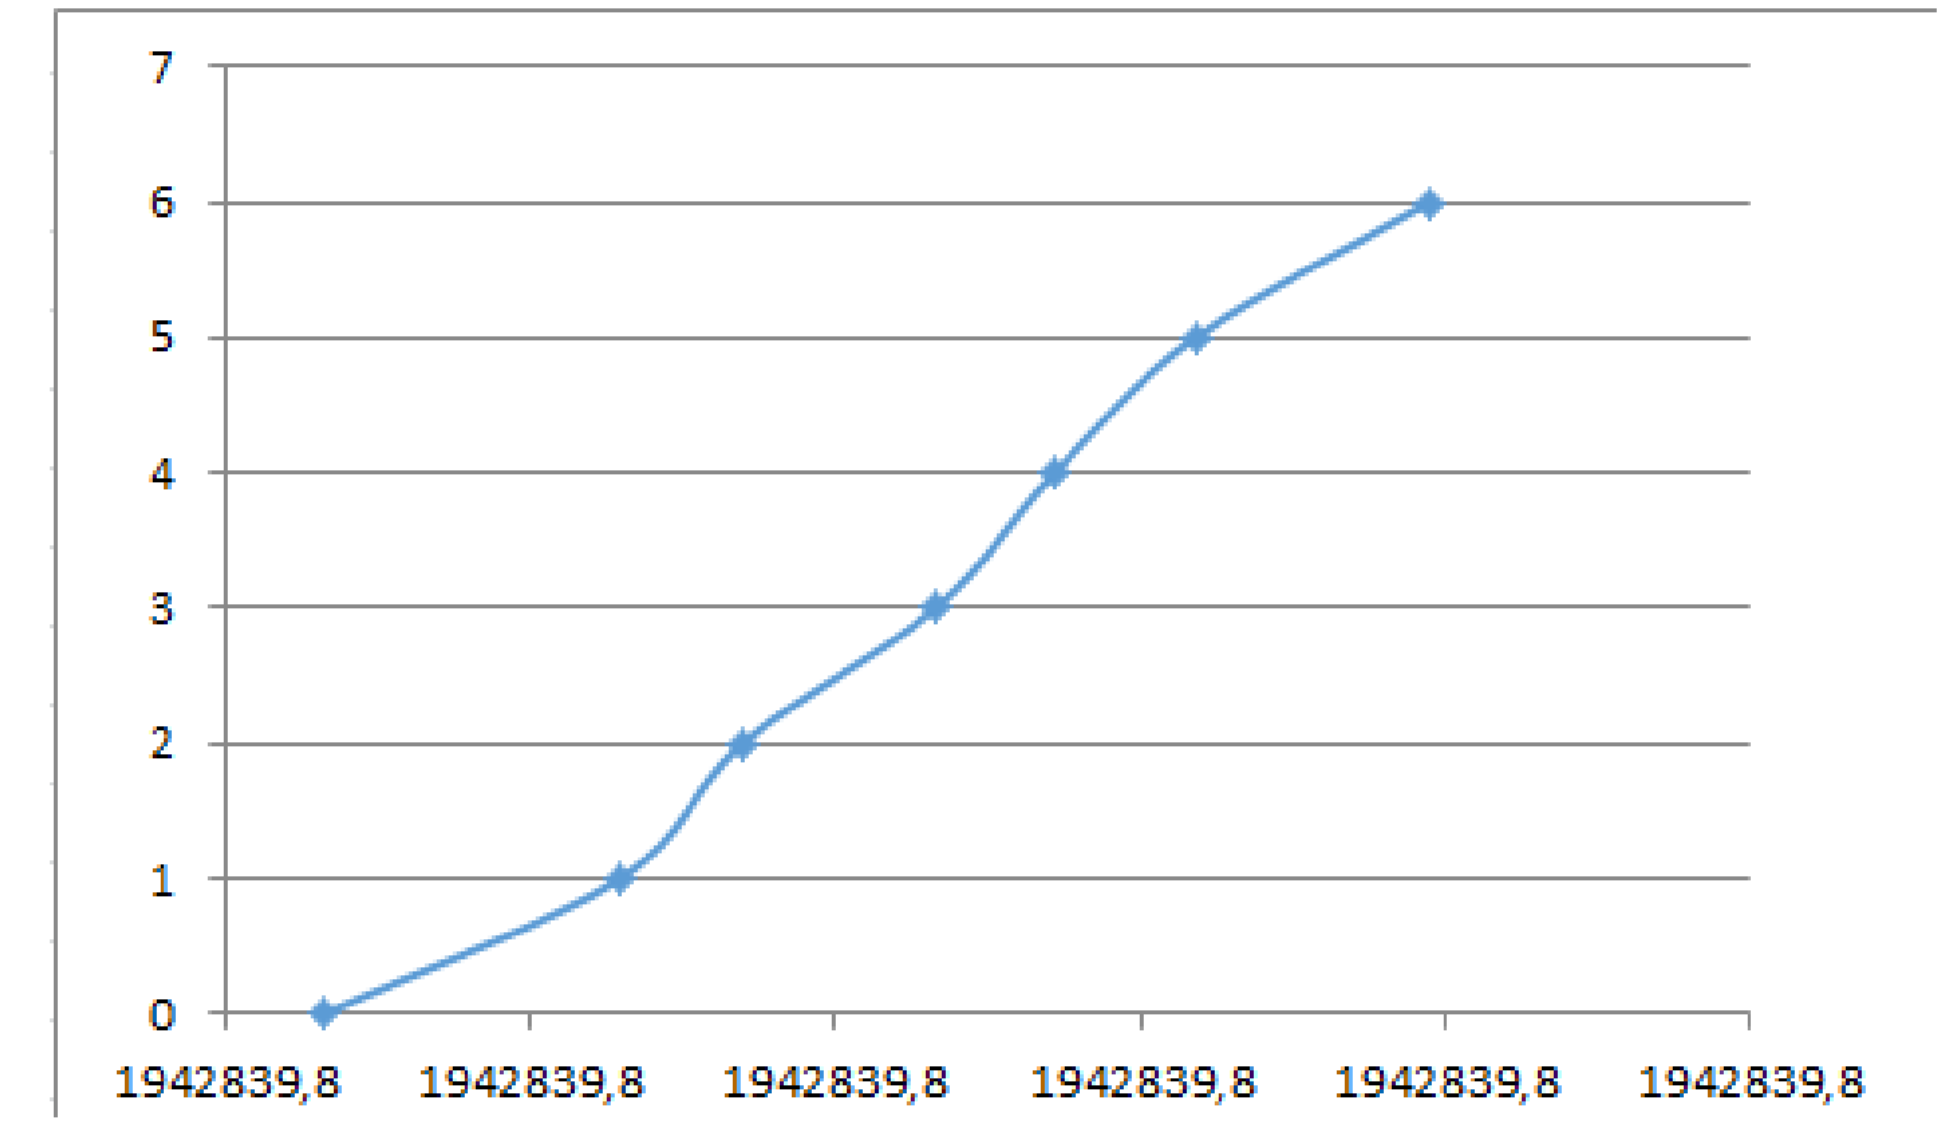
\includegraphics[scale = 0.25]{5-4.png}
    		    \caption{Время рассчёта 10 знакп после запятой в числе $\pi$}
                    \label{fig:my_label}
        		\end{figure}
        \section{Вывод}
        Мы исследвали то, как данные типа $float$ хранятся в памяти компьютера и обнаружили несколько интересных и важных в дальнейшем особенностей и ошибок. Научились визуализировать данные с помощью $Python$ и научились анализировать числа с плавающей точкой.
                

    \end{enumerate}
\end{document}
